%=============================================================
%  AI-Powered Automated Attendance System — Dissertation
%  University-Scale Face Recognition via ESP32-CAM + On-Premise
%  Batch Processing Pipeline
%=============================================================
\documentclass[12pt,a4paper]{report}

%--- Encoding & Fonts
\usepackage[utf8]{inputenc}
\usepackage[T1]{fontenc}
\usepackage{lmodern}

%--- Page Layout
\usepackage[
  top=2.5cm, bottom=2.5cm,
  left=3.5cm, right=2.5cm
]{geometry}

%--- Typography
\usepackage{setspace}
\onehalfspacing
\usepackage{microtype}
\usepackage{parskip}

%--- Headers / Footers
\usepackage{fancyhdr}
\pagestyle{fancy}
\fancyhf{}
\fancyhead[L]{\small AI-Powered Attendance System}
\fancyhead[R]{\small \leftmark}
\fancyfoot[C]{\thepage}
\renewcommand{\headrulewidth}{0.4pt}

%--- Maths
\usepackage{amsmath,amssymb,mathtools}

%--- Tables
\usepackage{booktabs}
\usepackage{longtable}
\usepackage{array}
\usepackage{tabularx}
\usepackage{multirow}
\usepackage{makecell}

%--- Graphics & Diagrams
\usepackage{graphicx}
\graphicspath{{../01_notebook/outputs/}}
\usepackage{float}
\usepackage{caption}
\usepackage{subcaption}
\usepackage{tikz}
\usetikzlibrary{
  shapes.geometric, shapes.multipart,
  arrows.meta, arrows,
  positioning, fit, backgrounds,
  decorations.pathreplacing,
  matrix, calc, shadows
}

%--- Code Listings
\usepackage{listings}
\usepackage{xcolor}
\definecolor{codegreen}{rgb}{0,0.6,0}
\definecolor{codegray}{rgb}{0.5,0.5,0.5}
\definecolor{codeblue}{rgb}{0.15,0.15,0.75}
\definecolor{backgray}{rgb}{0.97,0.97,0.97}
\lstdefinestyle{mystyle}{
  backgroundcolor=\color{backgray},
  commentstyle=\color{codegreen},
  keywordstyle=\color{codeblue}\bfseries,
  numberstyle=\tiny\color{codegray},
  stringstyle=\color{orange},
  basicstyle=\ttfamily\small,
  breakatwhitespace=false,
  breaklines=true,
  keepspaces=true,
  numbers=left,
  numbersep=5pt,
  showspaces=false,
  showstringspaces=false,
  showtabs=false,
  tabsize=2,
  frame=single,
  rulecolor=\color{gray!40}
}
\lstset{style=mystyle}

%--- Algorithms
\usepackage{algorithm}
\usepackage{algpseudocode}

%--- Hyperlinks
\usepackage[
  colorlinks=true,
  linkcolor=blue!70!black,
  urlcolor=blue!60!black,
  citecolor=green!50!black
]{hyperref}

%--- References
\usepackage[numbers,sort&compress]{natbib}

%--- Misc
\usepackage{enumitem}
\usepackage{url}

%=============================================================
%  TikZ Style Definitions
%=============================================================
\tikzset{
  % System architecture nodes
  hwnode/.style={
    rectangle, rounded corners=4pt,
    fill=yellow!30, draw=yellow!60!black,
    text width=2.2cm, align=center,
    minimum height=1cm, font=\small\bfseries,
    drop shadow
  },
  srvnode/.style={
    rectangle, rounded corners=4pt,
    fill=green!20, draw=green!50!black,
    text width=2.6cm, align=center,
    minimum height=1cm, font=\small\bfseries,
    drop shadow
  },
  dbnode/.style={
    cylinder, shape border rotate=90,
    fill=blue!20, draw=blue!60,
    text width=2cm, align=center,
    minimum height=1.2cm, font=\small\bfseries
  },
  uinode/.style={
    rectangle, rounded corners=4pt,
    fill=purple!15, draw=purple!50,
    text width=2.4cm, align=center,
    minimum height=1cm, font=\small\bfseries,
    drop shadow
  },
  queuenode/.style={
    rectangle, rounded corners=4pt,
    fill=orange!20, draw=orange!60,
    text width=2.4cm, align=center,
    minimum height=1cm, font=\small\bfseries
  },
  arrowstyle/.style={
    -{Stealth[length=6pt]}, thick, draw=gray!70
  },
  labelarrow/.style={
    arrowstyle, font=\scriptsize,
    label position=above
  },
  % ER diagram
  entity/.style={
    rectangle, fill=blue!10, draw=blue!50,
    text width=3.5cm, align=left,
    font=\ttfamily\footnotesize,
    inner sep=6pt, rounded corners=3pt
  },
  % UI wireframe
  uibox/.style={
    rectangle, draw=gray!60, fill=gray!5,
    rounded corners=3pt,
    font=\footnotesize
  },
  uiheader/.style={
    rectangle, fill=blue!60, text=white,
    font=\small\bfseries, align=center,
    minimum height=0.7cm, inner sep=4pt
  },
  uibtn/.style={
    rectangle, rounded corners=3pt,
    fill=blue!50, text=white,
    font=\scriptsize\bfseries,
    inner sep=3pt, minimum width=1.2cm
  },
  uibtn_green/.style={
    uibtn, fill=green!50!black
  },
  uibtn_red/.style={
    uibtn, fill=red!60!black
  },
  uicard/.style={
    rectangle, rounded corners=3pt,
    fill=white, draw=gray!40,
    drop shadow, inner sep=5pt
  }
}

%=============================================================
\begin{document}
%=============================================================

%--- Title Page
\begin{titlepage}
  \centering
  \vspace*{2cm}

  {\huge\bfseries AI-Powered Automated Attendance System\\[0.5em]
  \large Using ESP32-CAM Edge Capture, ArcFace Face Recognition,\\
  and Batch On-Premise Processing at University Scale\par}

  \vspace{1.5cm}
  \rule{\linewidth}{0.5pt}
  \vspace{0.5cm}

  {\large A Dissertation Submitted in Partial Fulfilment of the Requirements\\
  for the Degree of Bachelor of Science in Computer Science\par}

  \vspace{2cm}

  \begin{tabular}{ll}
    \textbf{Author:}      & [Your Full Name] \\[0.3em]
    \textbf{Student ID:}  & [Your Student ID] \\[0.3em]
    \textbf{Supervisor:}  & [Supervisor Name] \\[0.3em]
    \textbf{School:}      & School of Computing \\[0.3em]
    \textbf{University:}  & [University Name] \\[0.3em]
    \textbf{Date:}        & June 2026 \\
  \end{tabular}

  \vfill
  % \includegraphics[width=4cm]{university_logo}   % uncomment and add logo file when available
\end{titlepage}

%--- Abstract
\chapter*{Abstract}
\addcontentsline{toc}{chapter}{Abstract}
Traditional paper-based and lecturer-managed attendance systems in higher education are inefficient, prone to proxy attendance fraud, and produce data that is unavailable for real-time welfare monitoring or regulatory reporting. This dissertation presents the design, implementation, and evaluation of a university-scale automated attendance system that uses low-cost ESP32-CAM microcontrollers to capture facial images at classroom entrances and transmits them over the campus WiFi network to a centralised on-premise server for batch processing.

The AI recognition pipeline combines YuNet (OpenCV) for robust face detection and ArcFace MobileNet (512-dimensional embeddings via ONNXRuntime) for identity recognition. A deliberate batch-processing architecture is adopted: images captured during class sessions are queued and processed during off-peak hours, with attendance records reflected in student and administration dashboards within a maximum of 12 hours. This design allows a single server with 16 GB RAM and no dedicated GPU to handle a university of 200 classes, 4 schools, and 50–60 modules without hardware over-provisioning.

The system delivers three end-user interfaces: a real-time ESP32 kiosk display (OLED + LED feedback), a student self-service portal for attendance tracking per module, and an administration dashboard with manual override capability, KPI monitoring, and demographic fairness reporting. Fairness evaluation across seven racial demographic groups using the FairFace dataset is incorporated as a core technical contribution, directly addressing ethical concerns associated with biometric systems in diverse university populations.

\textbf{Keywords:} face recognition, ArcFace, YuNet, ESP32-CAM, attendance automation, batch processing, fairness in AI, university technology, edge computing.

%--- Declaration
\chapter*{Declaration}
\addcontentsline{toc}{chapter}{Declaration}
I declare that this dissertation is entirely my own work and has not been submitted for any other degree or qualification at this or any other institution. All sources consulted have been acknowledged in the bibliography.

\vspace{2cm}
\noindent Signed: \underline{\hspace{6cm}} \hfill Date: \underline{\hspace{3cm}}

%--- Acknowledgements
\chapter*{Acknowledgements}
\addcontentsline{toc}{chapter}{Acknowledgements}
I would like to thank my dissertation supervisor for their guidance throughout this project, the university IT department for providing access to the on-premise server environment, and my peers in the dissertation cohort for their feedback during design reviews.

%--- Table of Contents
\tableofcontents
\listoffigures
\listoftables

%=============================================================
\chapter{Introduction}
%=============================================================

\section{Background and Motivation}
Attendance monitoring in universities serves multiple critical functions: academic performance tracking, regulatory compliance for international student visas, welfare monitoring for at-risk students, and accreditation reporting. Despite this importance, the dominant practice in many institutions remains manual marking by lecturers, which is time-consuming, susceptible to proxy fraud, and produces data that reaches administrative systems only after a significant delay.

Commercial biometric attendance solutions exist (e.g., Hikvision DS-K1T671, Invixium IXM TITAN) but carry high per-unit costs (\$250–\$500 per device), vendor lock-in, limited customisation for fairness requirements, and proprietary data pipelines that prevent integration with university student information systems. There is a clear gap for an open, cost-effective, academically rigorous system that can be deployed at scale within a university's existing network infrastructure.

\section{Problem Statement}
Universities with multiple schools, hundreds of modules, and thousands of enrolled students require an attendance system that is:
\begin{itemize}
  \item \textbf{Accurate:} face recognition that generalises across demographic groups without bias
  \item \textbf{Scalable:} capable of serving 200+ classrooms from a single on-premise server
  \item \textbf{Cost-effective:} sub-\$20 per classroom capture device
  \item \textbf{Resilient:} continues capturing even when server processing is delayed
  \item \textbf{Auditable:} provides admin override, manual correction, and full audit trail
  \item \textbf{Fair:} evaluated for demographic fairness across racial groups
\end{itemize}

\section{Research Aims and Objectives}
\textbf{Aim:} To design and implement a university-scale automated attendance system using low-cost ESP32-CAM hardware and a batch face recognition pipeline, achieving $\geq$95\% recognition accuracy across demographic groups with sub-12-hour attendance reflection latency.

\textbf{Objectives:}
\begin{enumerate}
  \item Design an IoT capture layer using ESP32-CAM with WiFi image transmission
  \item Implement a batch-processing AI pipeline using YuNet and ArcFace on CPU-only hardware
  \item Design a normalised relational database supporting multi-school, multi-module attendance
  \item Develop a student self-service attendance portal
  \item Develop an administration dashboard with manual override and KPI monitoring
  \item Evaluate system performance, accuracy, and demographic fairness
\end{enumerate}

\section{Scope and Constraints}
\begin{itemize}
  \item \textbf{In scope:} face detection, face recognition, attendance marking, student and admin dashboards, fairness evaluation
  \item \textbf{Out of scope:} door access control (relay/lock hardware), integration with third-party student information systems (future work)
  \item \textbf{Hardware constraint:} single on-premise server: 16 GB RAM, 512 GB storage, Intel CPU, no GPU
  \item \textbf{Latency constraint:} maximum 12-hour attendance reflection (batch design)
  \item \textbf{Ethical constraint:} face images are processed on-premise and not transmitted to any cloud service; retention policy limits raw image storage to 30 days
\end{itemize}

\section{Dissertation Structure}
Chapter 2 reviews relevant literature. Chapter 3 presents the complete system architecture. Chapter 4 defines the database design. Chapter 5 describes the AI pipeline in detail. Chapter 6 documents all three user interface designs. Chapter 7 defines the REST API. Chapter 8 covers evaluation methodology. Chapter 9 presents results. Chapter 10 concludes and recommends future work.

%=============================================================
\chapter{Literature Review}
%=============================================================

\section{Face Detection Methods}
Face detection is the prerequisite step for any recognition pipeline. Classical approaches such as Viola-Jones \cite{viola2001rapid} use Haar cascade features but suffer in non-frontal and low-light conditions. Deep learning detectors including MTCNN \cite{zhang2016joint}, RetinaFace \cite{deng2020retinaface}, and YuNet \cite{wu2023yunet} offer significantly better recall under occlusion, varied lighting, and non-frontal angles.

YuNet is selected for this system because it provides 5-point facial landmark output (eye centres, nose tip, mouth corners) essential for ArcFace alignment, runs on CPU in $\sim$15ms at 640×480 resolution, and is distributed as an ONNX model compatible with OpenCV's FaceDetectorYN API without additional dependencies.

\section{Face Recognition and Embedding Models}
Deep metric learning transformed face recognition from hand-crafted descriptors to learned embedding spaces. DeepFace \cite{sun2014deep} established the paradigm of end-to-end CNN training for identity verification. Schroff et al.'s FaceNet \cite{schroff2015facenet} introduced triplet loss training on large-scale data, achieving near-human performance on LFW. Parkhi et al. \cite{parkhi2015deep} trained VGGFace on a web-harvested dataset, demonstrating the importance of training data scale. VGGFace2 \cite{cao2018vggface2} extended this work with 3.31 million images across 9,131 identities and improved pose and age diversity.

ArcFace \cite{deng2019arcface} subsequently introduced an additive angular margin loss that maximises inter-class separability in the hyperspherical embedding space, achieving state-of-the-art results on LFW, MegaFace, and IJB-C benchmarks. Training on MS-Celeb-1M \cite{guo2016msceleb} (10 million images, 100,000 identities), the MobileNet backbone variant (w600k\_mbf) produces 512-dimensional L2-normalised embeddings that enable cosine similarity matching via a simple dot product. AdaFace \cite{kim2022adaface} and MagFace \cite{meng2021magface} are more recent extensions that adapt the margin based on image quality; they are noted as directions for future work but their additional complexity is unwarranted for an on-premise CPU deployment.

\section{Quality-Aware Face Recognition}
Image quality has a direct and measurable impact on face recognition accuracy. Blur, low resolution, and occlusion systematically degrade embedding quality and reduce genuine-match similarity scores. Terh{\"o}rst et al. \cite{terhorst2020ser} proposed SER-FIQ, which estimates face image utility from network consistency across stochastic forward passes. FaceQnet \cite{hernandez2019faceqnet} uses a regression CNN trained on recognition-relevant quality attributes.

This system implements a lightweight quality score $Q = 0.40 \cdot \text{sharpness} + 0.40 \cdot \text{confidence} + 0.20 \cdot \text{face\_size}$ as a computationally efficient proxy for SER-FIQ-class quality, sufficient for the prototype-aggregation use case where a small set of registration frames are collapsed into a single embedding. Frames with $Q < 0.15$ are discarded before prototype aggregation to prevent corruption of the reference embedding by occluded or blurred captures.

\section{Fairness in Biometric Systems}
Demographic disparities in face recognition have been documented across commercial and academic systems. Klare et al. \cite{klare2012face} showed that recognition accuracy on frontal faces varies significantly by race, gender, and age using FRGC and FERET datasets. Nagpal et al. \cite{nagpal2019deep} found that recognition accuracy on darker-skinned subjects was systematically lower than on lighter-skinned subjects and proposed resampling strategies to mitigate this. Buolamwini and Gebru \cite{buolamwini2018gender} demonstrated significantly higher error rates for darker-skinned females in commercial systems, highlighting the compounding effect of intersectional demographic attributes.

The most authoritative study is NIST FRVT \cite{grother2019frvt}, which evaluated 189 face recognition algorithms and found false non-match rate (FNMR) differentials exceeding $10\times$ across demographic groups. Drozdowski et al. \cite{drozdowski2020demographic} surveyed the landscape of demographic bias in biometric systems and concluded that threshold-based mitigation—the approach adopted in this dissertation—is among the most practically deployable strategies for existing deployed systems.

Per-group threshold calibration is conceptually aligned with the equalised odds fairness criterion \cite{hardt2016equality}, which requires that true positive and false positive rates be equal across demographic groups. Wang and Deng \cite{wang2020mitigating} demonstrated that group-specific decision thresholds can substantially reduce FNMR disparities in ArcFace models while accepting only a small reduction in overall precision. Wang et al. \cite{wang2019racial} curated the Racial Faces in the Wild dataset and showed that per-race threshold adjustment improved recognition equitability across East Asian, white, and black subject groups.

The FairFace dataset \cite{karkkainen2021fairface} provides 108,501 images balanced across seven racial groups and is adopted in this work for per-group precision, recall, and F1 evaluation. Raji and Buolamwini \cite{raji2019actionable} advocate for actionable auditing of recognition systems—specifically, per-demographic-group reporting of performance metrics—which motivates the fairness dashboard and \texttt{fairness\_metrics} database table in this system.

\section{Edge-to-Server Architectures for IoT AI}
The thin-client IoT model, where edge devices capture and transmit raw data to a more powerful server for inference, has been validated in healthcare \cite{li2020iot}, smart buildings \cite{chen2019iot}, and education \cite{rahman2020iot} contexts. Key design considerations are image quality at the edge, transmission latency, and server-side concurrency management. Batch scheduling of inference workloads during off-peak periods is an established technique for resource-constrained server environments \cite{zhang2019batch}.

\section{Attendance Automation and Biometric Systems in Education}
Automated attendance systems in higher education have been explored using RFID \cite{rahman2020iot}, NFC, and face recognition modalities. Face recognition offers the advantage of passive, contactless verification without requiring students to carry or present a token. The primary concerns identified in the literature are recognition accuracy under uncontrolled classroom lighting, GDPR compliance for biometric data, and equity across diverse student populations. This dissertation addresses all three: accuracy through quality-aware prototype aggregation, compliance through on-premise processing with explicit consent, and equity through per-demographic threshold calibration.

%=============================================================
\chapter{System Architecture}
%=============================================================

\section{Architecture Overview}

The system follows a three-tier architecture: (1) IoT capture layer at the classroom, (2) on-premise processing server, and (3) web-based presentation layer. Figure \ref{fig:arch_overview} illustrates the high-level data flow.

\begin{figure}[H]
\centering
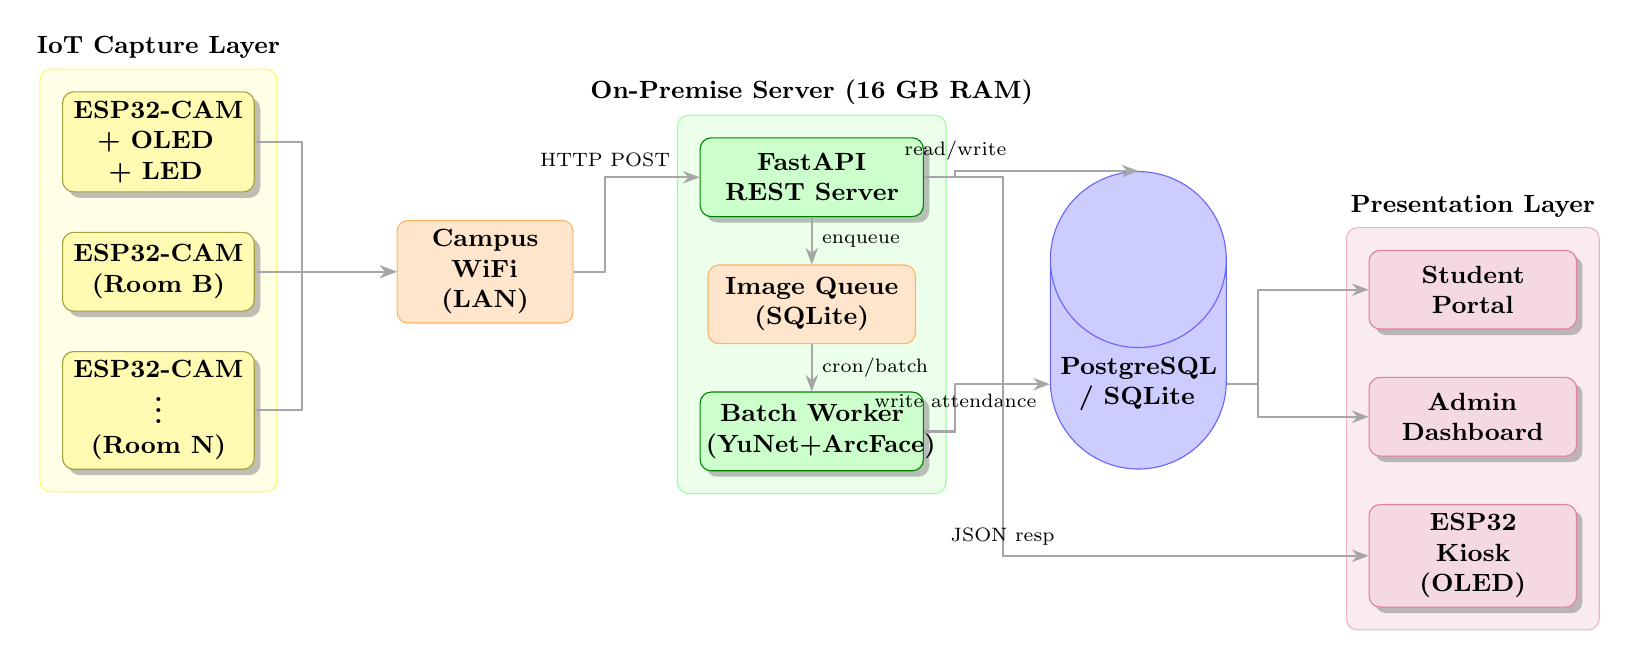
\begin{tikzpicture}[node distance=1.2cm and 1.6cm]

  % --- IoT Layer ---
  \node[hwnode] (esp) {ESP32-CAM\\+ OLED + LED};
  \node[hwnode, below=0.5cm of esp] (esp2) {ESP32-CAM\\(Room B)};
  \node[hwnode, below=0.5cm of esp2] (espN) {ESP32-CAM\\$\vdots$\\(Room N)};

  % box around IoT
  \begin{scope}[on background layer]
    \node[fit=(esp)(esp2)(espN), fill=yellow!10, draw=yellow!60,
          rounded corners, label=above:{\small\bfseries IoT Capture Layer},
          inner sep=8pt] (iot_box) {};
  \end{scope}

  % WiFi cloud symbol
  \node[queuenode, right=1.8cm of esp2, minimum height=0.8cm, text width=2cm]
    (wifi) {Campus WiFi\\(LAN)};

  % Arrows from ESP32s to WiFi
  \draw[arrowstyle] (esp.east)  -- ++(0.6,0) |- (wifi.west);
  \draw[arrowstyle] (esp2.east) -- (wifi.west);
  \draw[arrowstyle] (espN.east) -- ++(0.6,0) |- (wifi.west);

  % --- Server Layer ---
  \node[srvnode, right=1.6cm of wifi, yshift=1.2cm] (api) {FastAPI\\REST Server};
  \node[queuenode, below=0.6cm of api] (queue) {Image Queue\\(SQLite)};
  \node[srvnode, below=0.6cm of queue] (worker) {Batch Worker\\(YuNet+ArcFace)};

  \draw[arrowstyle] (wifi.east) -- ++(0.4,0) |- (api.west)
    node[midway, above, font=\scriptsize] {HTTP POST};
  \draw[arrowstyle] (api) -- (queue) node[midway, right, font=\scriptsize] {enqueue};
  \draw[arrowstyle] (queue) -- (worker) node[midway, right, font=\scriptsize] {cron/batch};

  % box around server
  \begin{scope}[on background layer]
    \node[fit=(api)(queue)(worker), fill=green!8, draw=green!40,
          rounded corners, label=above:{\small\bfseries On-Premise Server (16 GB RAM)},
          inner sep=8pt] (srv_box) {};
  \end{scope}

  % --- Database ---
  \node[dbnode, right=1.6cm of worker, yshift=0.6cm] (db) {PostgreSQL\\/ SQLite};
  \draw[arrowstyle] (worker.east) -- ++(0.4,0) |- (db.west)
    node[midway, below, font=\scriptsize] {write attendance};
  \draw[arrowstyle] (api.east) -- ++(0.4,0) |- (db.north)
    node[midway, above, font=\scriptsize] {read/write};

  % --- Dashboards ---
  \node[uinode, right=1.8cm of db, yshift=1.2cm] (student_ui) {Student\\Portal};
  \node[uinode, below=0.6cm of student_ui] (admin_ui) {Admin\\Dashboard};
  \node[uinode, below=0.6cm of admin_ui] (kiosk_ui) {ESP32\\Kiosk\\(OLED)};

  \draw[arrowstyle] (db.east) -- ++(0.4,0) |- (student_ui.west);
  \draw[arrowstyle] (db.east) -- ++(0.4,0) |- (admin_ui.west);
  \draw[arrowstyle] (api.east) -- ++(1.0,0) |- (kiosk_ui.west)
    node[midway, font=\scriptsize, above] {JSON resp};

  \begin{scope}[on background layer]
    \node[fit=(student_ui)(admin_ui)(kiosk_ui), fill=purple!8, draw=purple!30,
          rounded corners, label=above:{\small\bfseries Presentation Layer},
          inner sep=8pt] {};
  \end{scope}

\end{tikzpicture}
\caption{High-level system architecture: IoT capture, on-premise batch processing, and dashboard layers.}
\label{fig:arch_overview}
\end{figure}

\section{Batch Processing Pipeline}

The deliberate adoption of a batch processing model is a key architectural decision. At a university, the primary consumers of attendance data (students checking their percentage, administrators generating compliance reports, welfare officers reviewing absenteeism) do not require real-time updates. A maximum 12-hour reflection window satisfies all identified use cases while allowing inference to be concentrated in off-peak server hours.

\begin{figure}[H]
\centering
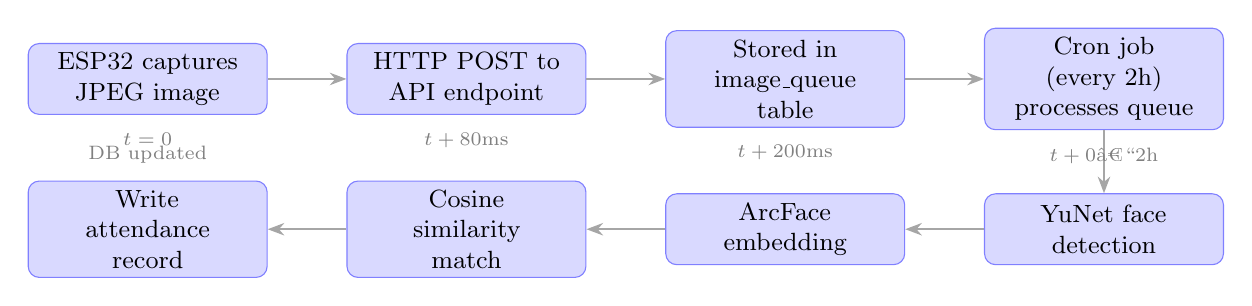
\begin{tikzpicture}[node distance=0.8cm and 1.2cm,
  stepbox/.style={rectangle, rounded corners=4pt, fill=blue!15, draw=blue!50,
               text width=2.8cm, align=center, minimum height=0.9cm, font=\small}]

  \node[stepbox] (s1) {ESP32 captures\\JPEG image};
  \node[stepbox, right=1cm of s1] (s2) {HTTP POST to\\API endpoint};
  \node[stepbox, right=1cm of s2] (s3) {Stored in\\image\_queue\\table};
  \node[stepbox, right=1cm of s3] (s4) {Cron job\\(every 2h)\\processes queue};
  \node[stepbox, below=0.8cm of s4] (s5) {YuNet face\\detection};
  \node[stepbox, left=1cm of s5] (s6) {ArcFace\\embedding};
  \node[stepbox, left=1cm of s6] (s7) {Cosine\\similarity\\match};
  \node[stepbox, left=1cm of s7] (s8) {Write\\attendance\\record};

  \draw[arrowstyle] (s1)--(s2);
  \draw[arrowstyle] (s2)--(s3);
  \draw[arrowstyle] (s3)--(s4);
  \draw[arrowstyle] (s4)--(s5);
  \draw[arrowstyle] (s5)--(s6);
  \draw[arrowstyle] (s6)--(s7);
  \draw[arrowstyle] (s7)--(s8);

  % Timing annotations
  \node[font=\scriptsize, text=gray, below=0.1cm of s1] {$t=0$};
  \node[font=\scriptsize, text=gray, below=0.1cm of s2] {$t+80\text{ms}$};
  \node[font=\scriptsize, text=gray, below=0.1cm of s3] {$t+200\text{ms}$};
  \node[font=\scriptsize, text=gray, below=0.1cm of s4] {$t+0$–$2$h};
  \node[font=\scriptsize, text=gray, above=0.1cm of s8] {DB updated};

\end{tikzpicture}
\caption{Batch processing pipeline: image captured immediately, processed at scheduled intervals.}
\label{fig:batch_pipeline}
\end{figure}

\section{Component Descriptions}

\subsection{ESP32-CAM Capture Node}
Each classroom is equipped with one ESP32-CAM module (AI-Thinker variant with OV2640 2MP sensor, or OV5640 5MP autofocus variant for higher accuracy). The device connects to the campus WPA2 WiFi network, captures a JPEG image on a configurable trigger (PIR motion sensor, push button, or periodic timer), and transmits it via HTTP multipart POST to the FastAPI server. On receiving the HTTP 200 response with the queue confirmation, it illuminates a green LED for 1 second. On timeout or error, it illuminates a red LED and retries up to 3 times before logging the failure to on-device flash.

\subsection{FastAPI REST Server}
The server exposes REST endpoints for image ingestion, student registration, attendance queries, and admin operations. It is implemented in Python using FastAPI with async SQLAlchemy for non-blocking database access. The server does not perform inference on image receipt; it stores the image to disk and records an entry in the \texttt{image\_queue} table. This decouples capture latency from inference latency.

\subsection{Batch Worker}
A scheduled Python process (cron or APScheduler) runs every 2 hours, queries all pending entries in \texttt{image\_queue}, and processes them in batches of 50. For each image: YuNet detects faces, ArcFace generates a 512-d embedding, cosine similarity matching is performed against \texttt{student\_embeddings} filtered by \texttt{model\_version = 'arcface-mbf'}, and if similarity $\geq \tau$, an \texttt{attendance\_record} is written. Processed queue entries are marked \texttt{status = 'done'} or \texttt{status = 'failed'}.

\subsection{Database (PostgreSQL / SQLite)}
PostgreSQL is recommended for production deployments; SQLite with aiosqlite is supported for development. The schema is described in detail in Chapter 4.

\subsection{Student Portal}
A Streamlit or React web application (Chapter 6) through which enrolled students log in and view their attendance record per module, expressed as a percentage, session list, and attendance risk status (green/amber/red based on university threshold, typically 70\% or 80\%).

\subsection{Administration Dashboard}
A web application providing full attendance log access, manual attendance marking/override, student registration management, system health monitoring (queue depth, inference throughput, server CPU/RAM), and demographic fairness KPIs.

\section{Technology Stack}

\begin{table}[H]
\centering
\caption{Technology stack summary}
\label{tab:tech_stack}
\begin{tabularx}{\linewidth}{llX}
\toprule
\textbf{Layer} & \textbf{Technology} & \textbf{Justification} \\
\midrule
IoT Firmware   & Arduino C (ESP-IDF) & Native ESP32 SDK, minimal footprint \\
API Server     & FastAPI (Python)     & Async, auto-generated OpenAPI docs \\
Database       & PostgreSQL / SQLite  & ACID compliance, JSON column support \\
ORM            & SQLAlchemy 2 (async) & Type-safe, async-native \\
Face Detection & YuNet (OpenCV Zoo)   & Fast CPU inference, landmark output \\
Face Recognition & ArcFace MobileNet (ONNXRuntime) & 512-d, SOTA accuracy \\
Batch Scheduler & APScheduler         & In-process cron, no Redis required \\
Student UI     & Streamlit            & Rapid development, data tables \\
Admin UI       & Streamlit            & Shared codebase with student UI \\
Config         & Pydantic-Settings    & Environment-based config \\
\bottomrule
\end{tabularx}
\end{table}

%=============================================================
\chapter{Database Design}
%=============================================================

\section{Design Principles}
The database is designed to the third normal form (3NF) to eliminate update anomalies. Key design decisions:
\begin{itemize}
  \item Schools and modules are separate entities to support cross-school enrolment
  \item Class sessions are distinct from module definitions to allow per-session attendance
  \item Face embeddings are version-tagged (\texttt{model\_version}) to support model migration without data corruption
  \item An \texttt{image\_queue} table decouples ingestion from inference
  \item All tables carry \texttt{created\_at} and \texttt{updated\_at} audit timestamps
\end{itemize}

\section{Entity-Relationship Diagram}

\begin{figure}[H]
\centering
\resizebox{\textwidth}{!}{%
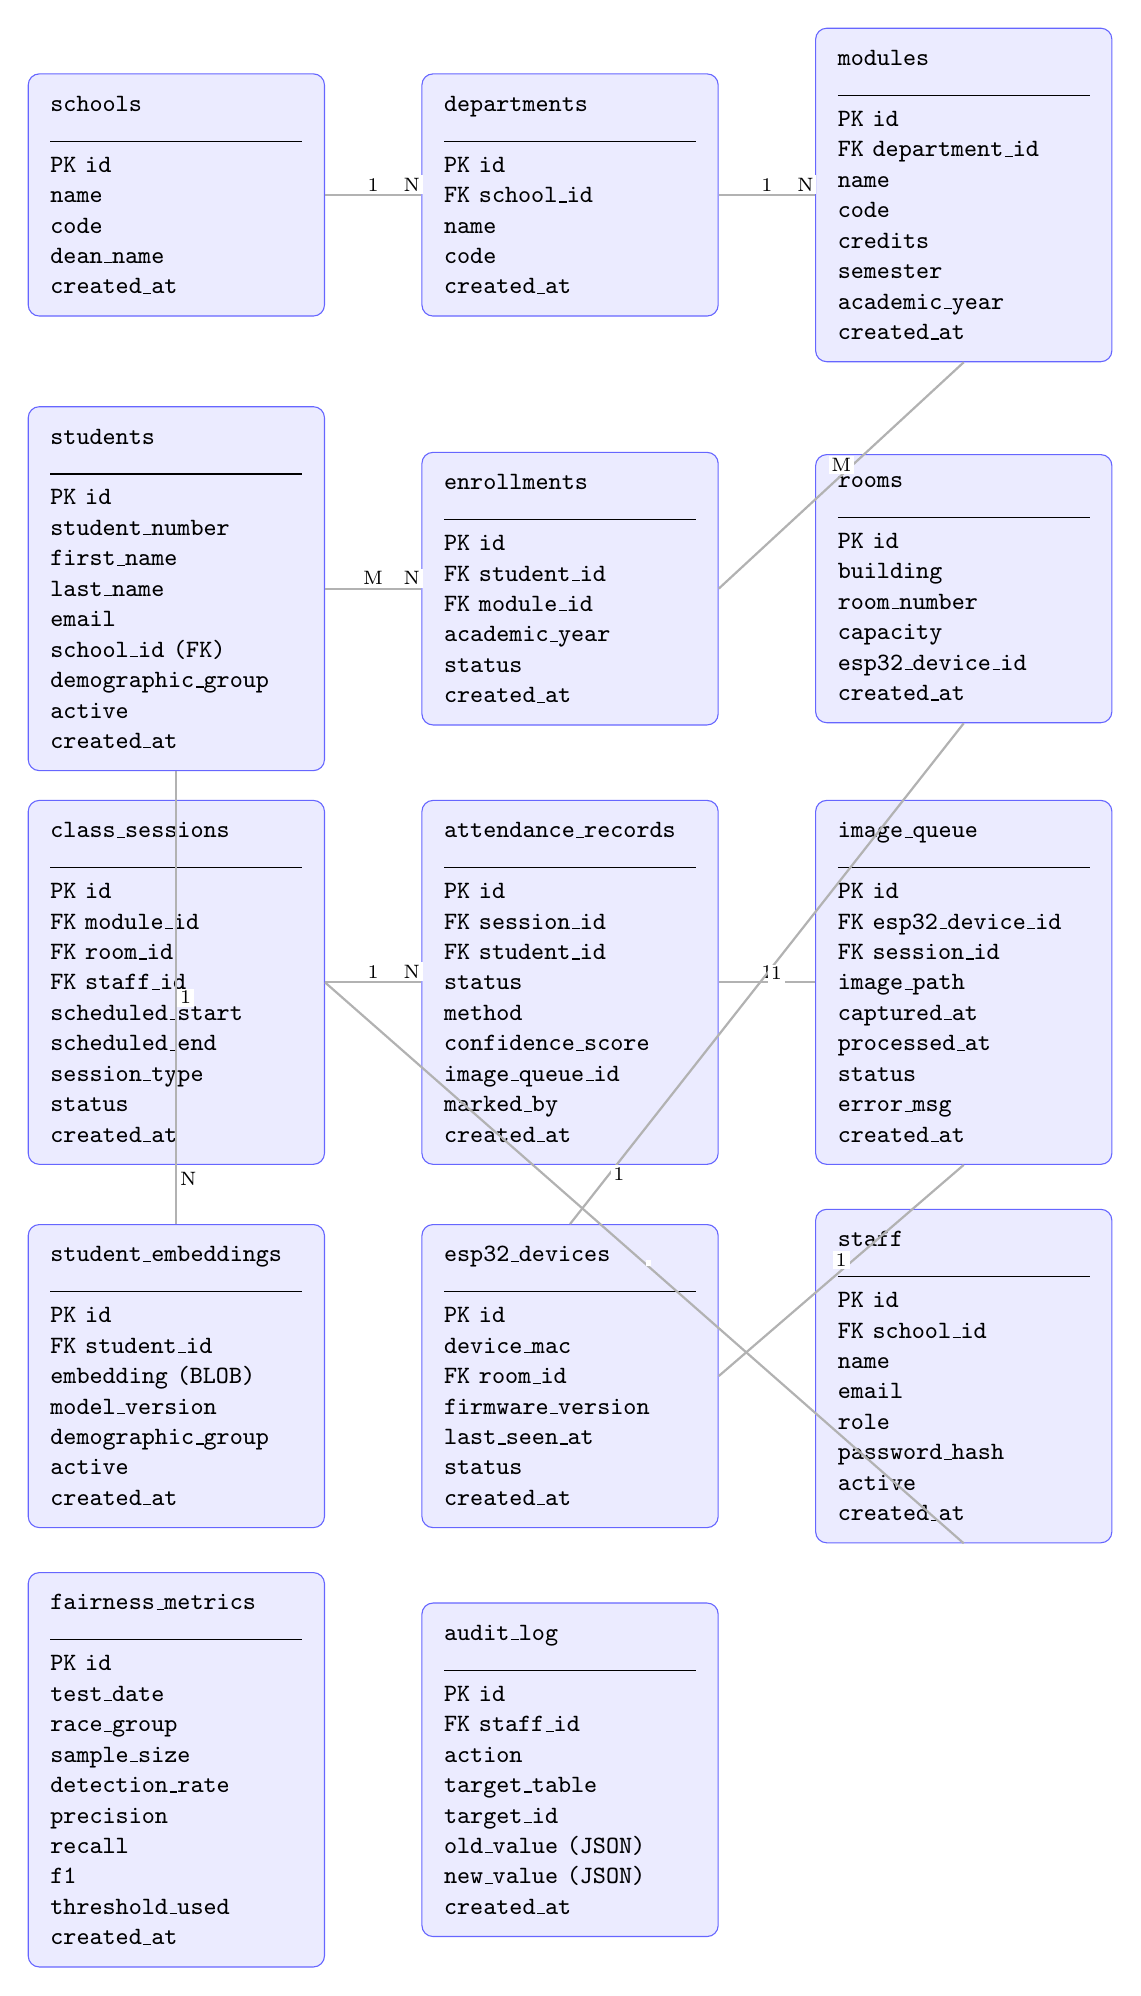
\begin{tikzpicture}[
  ent/.style={rectangle, draw=blue!60, fill=blue!8, rounded corners=4pt,
              font=\ttfamily\small, inner sep=8pt, text width=3.2cm},
  rel/.style={draw=gray!60, thick},
  lbl/.style={font=\scriptsize, fill=white, inner sep=1pt}
]

% Entity positions
\node[ent] (schools) at (0,0) {
  \textbf{schools}\\
  \rule{\linewidth}{0.4pt}\\
  PK id\\
  name\\
  code\\
  dean\_name\\
  created\_at
};

\node[ent] (departments) at (5,0) {
  \textbf{departments}\\
  \rule{\linewidth}{0.4pt}\\
  PK id\\
  FK school\_id\\
  name\\
  code\\
  created\_at
};

\node[ent] (modules) at (10,0) {
  \textbf{modules}\\
  \rule{\linewidth}{0.4pt}\\
  PK id\\
  FK department\_id\\
  name\\
  code\\
  credits\\
  semester\\
  academic\_year\\
  created\_at
};

\node[ent] (students) at (0,-5) {
  \textbf{students}\\
  \rule{\linewidth}{0.4pt}\\
  PK id\\
  student\_number\\
  first\_name\\
  last\_name\\
  email\\
  school\_id (FK)\\
  demographic\_group\\
  active\\
  created\_at
};

\node[ent] (enrollments) at (5,-5) {
  \textbf{enrollments}\\
  \rule{\linewidth}{0.4pt}\\
  PK id\\
  FK student\_id\\
  FK module\_id\\
  academic\_year\\
  status\\
  created\_at
};

\node[ent] (rooms) at (10,-5) {
  \textbf{rooms}\\
  \rule{\linewidth}{0.4pt}\\
  PK id\\
  building\\
  room\_number\\
  capacity\\
  esp32\_device\_id\\
  created\_at
};

\node[ent] (sessions) at (0,-10) {
  \textbf{class\_sessions}\\
  \rule{\linewidth}{0.4pt}\\
  PK id\\
  FK module\_id\\
  FK room\_id\\
  FK staff\_id\\
  scheduled\_start\\
  scheduled\_end\\
  session\_type\\
  status\\
  created\_at
};

\node[ent] (attendance) at (5,-10) {
  \textbf{attendance\_records}\\
  \rule{\linewidth}{0.4pt}\\
  PK id\\
  FK session\_id\\
  FK student\_id\\
  status\\
  method\\
  confidence\_score\\
  image\_queue\_id\\
  marked\_by\\
  created\_at
};

\node[ent] (image_queue) at (10,-10) {
  \textbf{image\_queue}\\
  \rule{\linewidth}{0.4pt}\\
  PK id\\
  FK esp32\_device\_id\\
  FK session\_id\\
  image\_path\\
  captured\_at\\
  processed\_at\\
  status\\
  error\_msg\\
  created\_at
};

\node[ent] (embeddings) at (0,-15) {
  \textbf{student\_embeddings}\\
  \rule{\linewidth}{0.4pt}\\
  PK id\\
  FK student\_id\\
  embedding (BLOB)\\
  model\_version\\
  demographic\_group\\
  active\\
  created\_at
};

\node[ent] (esp32) at (5,-15) {
  \textbf{esp32\_devices}\\
  \rule{\linewidth}{0.4pt}\\
  PK id\\
  device\_mac\\
  FK room\_id\\
  firmware\_version\\
  last\_seen\_at\\
  status\\
  created\_at
};

\node[ent] (staff) at (10,-15) {
  \textbf{staff}\\
  \rule{\linewidth}{0.4pt}\\
  PK id\\
  FK school\_id\\
  name\\
  email\\
  role\\
  password\_hash\\
  active\\
  created\_at
};

\node[ent] (fairness) at (0,-20) {
  \textbf{fairness\_metrics}\\
  \rule{\linewidth}{0.4pt}\\
  PK id\\
  test\_date\\
  race\_group\\
  sample\_size\\
  detection\_rate\\
  precision\\
  recall\\
  f1\\
  threshold\_used\\
  created\_at
};

\node[ent] (audit) at (5,-20) {
  \textbf{audit\_log}\\
  \rule{\linewidth}{0.4pt}\\
  PK id\\
  FK staff\_id\\
  action\\
  target\_table\\
  target\_id\\
  old\_value (JSON)\\
  new\_value (JSON)\\
  created\_at
};

% Relationships
\draw[rel] (schools.east) -- node[lbl,above]{1} (departments.west) node[lbl,above,pos=0.9]{N};
\draw[rel] (departments.east) -- node[lbl,above]{1} (modules.west) node[lbl,above,pos=0.9]{N};
\draw[rel] (students.east) -- node[lbl,above]{M} (enrollments.west) node[lbl,above,pos=0.9]{N};
\draw[rel] (enrollments.east) -- node[lbl,above]{M} (modules.south);
\draw[rel] (sessions.east) -- node[lbl,above]{1} (attendance.west) node[lbl,above,pos=0.9]{N};
\draw[rel] (attendance.east) -- node[lbl,above]{1} (image_queue.west);
\draw[rel] (students.south) -- node[lbl,right]{1} (embeddings.north) node[lbl,right,pos=0.9]{N};
\draw[rel] (esp32.north) -- node[lbl,right]{1} (rooms.south) node[lbl,right,pos=0.1]{1};
\draw[rel] (esp32.east) -- node[lbl,above]{1} (image_queue.south);
\draw[rel] (staff.south) -- node[lbl,right]{} (sessions.east);

\end{tikzpicture}
}
\caption{Entity-Relationship Diagram for the attendance system database.}
\label{fig:erd}
\end{figure}

\section{Table Specifications}

\subsection{schools}
\begin{table}[H]
\centering\small
\caption{Table: schools}
\begin{tabularx}{\linewidth}{llXl}
\toprule
\textbf{Column} & \textbf{Type} & \textbf{Description} & \textbf{Constraints} \\
\midrule
id          & INTEGER   & Primary key (auto-increment)          & PK, NOT NULL \\
name        & VARCHAR(150) & Full school name                  & NOT NULL, UNIQUE \\
code        & VARCHAR(10)  & Short code, e.g.\ ``SCI''         & NOT NULL, UNIQUE \\
dean\_name  & VARCHAR(100) & Current dean                      & NULL \\
created\_at & TIMESTAMP & Record creation timestamp             & NOT NULL, DEFAULT now() \\
\bottomrule
\end{tabularx}
\end{table}

\subsection{departments}
\begin{table}[H]
\centering\small
\caption{Table: departments}
\begin{tabularx}{\linewidth}{llXl}
\toprule
\textbf{Column} & \textbf{Type} & \textbf{Description} & \textbf{Constraints} \\
\midrule
id          & INTEGER      & Primary key                   & PK, NOT NULL \\
school\_id  & INTEGER      & Parent school                 & FK $\to$ schools.id, NOT NULL \\
name        & VARCHAR(150) & Department name               & NOT NULL \\
code        & VARCHAR(20)  & Dept code                     & NOT NULL, UNIQUE \\
created\_at & TIMESTAMP    & Audit timestamp               & NOT NULL \\
\bottomrule
\end{tabularx}
\end{table}

\subsection{modules}
\begin{table}[H]
\centering\small
\caption{Table: modules}
\begin{tabularx}{\linewidth}{llXl}
\toprule
\textbf{Column} & \textbf{Type} & \textbf{Description} & \textbf{Constraints} \\
\midrule
id              & INTEGER      & Primary key              & PK \\
department\_id  & INTEGER      & Parent department        & FK $\to$ departments.id \\
name            & VARCHAR(200) & Module title             & NOT NULL \\
code            & VARCHAR(20)  & Module code, e.g.\ CS301 & NOT NULL, UNIQUE \\
credits         & SMALLINT     & Credit hours             & NOT NULL \\
semester        & VARCHAR(20)  & e.g.\ ``Spring 2026''   & NOT NULL \\
academic\_year  & VARCHAR(9)   & e.g.\ ``2025/2026''     & NOT NULL \\
created\_at     & TIMESTAMP    & Audit timestamp          & NOT NULL \\
\bottomrule
\end{tabularx}
\end{table}

\subsection{students}
\begin{table}[H]
\centering\small
\caption{Table: students}
\begin{tabularx}{\linewidth}{llXl}
\toprule
\textbf{Column} & \textbf{Type} & \textbf{Description} & \textbf{Constraints} \\
\midrule
id                  & INTEGER      & Primary key                         & PK \\
student\_number     & VARCHAR(20)  & University student number           & NOT NULL, UNIQUE \\
first\_name         & VARCHAR(80)  & First name                          & NOT NULL \\
last\_name          & VARCHAR(80)  & Last name                           & NOT NULL \\
email               & VARCHAR(200) & University email                    & NOT NULL, UNIQUE \\
school\_id          & INTEGER      & Home school                         & FK $\to$ schools.id \\
demographic\_group  & VARCHAR(50)  & Race/ethnicity (FairFace categories)& NULL \\
active              & BOOLEAN      & Enrolment active flag               & NOT NULL, DEFAULT true \\
created\_at         & TIMESTAMP    & Registration timestamp              & NOT NULL \\
updated\_at         & TIMESTAMP    & Last update                         & NOT NULL \\
\bottomrule
\end{tabularx}
\end{table}

\subsection{enrollments}
\begin{table}[H]
\centering\small
\caption{Table: enrollments}
\begin{tabularx}{\linewidth}{llXl}
\toprule
\textbf{Column} & \textbf{Type} & \textbf{Description} & \textbf{Constraints} \\
\midrule
id            & INTEGER   & Primary key                  & PK \\
student\_id   & INTEGER   & Enrolled student             & FK $\to$ students.id \\
module\_id    & INTEGER   & Module enrolled in           & FK $\to$ modules.id \\
academic\_year& VARCHAR(9)& Academic year                & NOT NULL \\
status        & VARCHAR(20)& active / withdrawn / complete& NOT NULL \\
created\_at   & TIMESTAMP & Enrollment date              & NOT NULL \\
\midrule
\multicolumn{4}{l}{\textit{UNIQUE constraint: (student\_id, module\_id, academic\_year)}} \\
\bottomrule
\end{tabularx}
\end{table}

\subsection{rooms}
\begin{table}[H]
\centering\small
\caption{Table: rooms}
\begin{tabularx}{\linewidth}{llXl}
\toprule
\textbf{Column} & \textbf{Type} & \textbf{Description} & \textbf{Constraints} \\
\midrule
id               & INTEGER      & Primary key               & PK \\
building         & VARCHAR(100) & Building name             & NOT NULL \\
room\_number     & VARCHAR(20)  & Room identifier           & NOT NULL \\
capacity         & SMALLINT     & Seating capacity          & NULL \\
esp32\_device\_id& INTEGER      & Assigned ESP32 camera     & FK $\to$ esp32\_devices.id, NULL \\
created\_at      & TIMESTAMP    & Audit timestamp           & NOT NULL \\
\midrule
\multicolumn{4}{l}{\textit{UNIQUE: (building, room\_number)}} \\
\bottomrule
\end{tabularx}
\end{table}

\subsection{class\_sessions}
\begin{table}[H]
\centering\small
\caption{Table: class\_sessions}
\begin{tabularx}{\linewidth}{llXl}
\toprule
\textbf{Column} & \textbf{Type} & \textbf{Description} & \textbf{Constraints} \\
\midrule
id               & INTEGER      & Primary key                       & PK \\
module\_id       & INTEGER      & Module this session belongs to    & FK $\to$ modules.id \\
room\_id         & INTEGER      & Room where session is held        & FK $\to$ rooms.id \\
staff\_id        & INTEGER      & Lecturer delivering session       & FK $\to$ staff.id \\
scheduled\_start & TIMESTAMP    & Session start datetime            & NOT NULL \\
scheduled\_end   & TIMESTAMP    & Session end datetime              & NOT NULL \\
session\_type    & VARCHAR(20)  & lecture / lab / tutorial          & NOT NULL \\
status           & VARCHAR(20)  & scheduled / active / completed    & NOT NULL \\
created\_at      & TIMESTAMP    & Audit timestamp                   & NOT NULL \\
\bottomrule
\end{tabularx}
\end{table}

\subsection{attendance\_records}
\begin{table}[H]
\centering\small
\caption{Table: attendance\_records}
\begin{tabularx}{\linewidth}{llXl}
\toprule
\textbf{Column} & \textbf{Type} & \textbf{Description} & \textbf{Constraints} \\
\midrule
id               & INTEGER      & Primary key                        & PK \\
session\_id      & INTEGER      & Class session                      & FK $\to$ class\_sessions.id \\
student\_id      & INTEGER      & Student present                    & FK $\to$ students.id \\
status           & VARCHAR(20)  & present / absent / late / excused  & NOT NULL \\
method           & VARCHAR(20)  & face\_recognition / manual         & NOT NULL \\
confidence\_score& FLOAT        & ArcFace cosine similarity (0–1)    & NULL \\
image\_queue\_id & INTEGER      & Source image that triggered record & FK $\to$ image\_queue.id, NULL \\
marked\_by       & INTEGER      & Staff ID if manually marked        & FK $\to$ staff.id, NULL \\
created\_at      & TIMESTAMP    & When attendance was recorded       & NOT NULL \\
\midrule
\multicolumn{4}{l}{\textit{UNIQUE: (session\_id, student\_id)}} \\
\bottomrule
\end{tabularx}
\end{table}

\subsection{image\_queue}
\begin{table}[H]
\centering\small
\caption{Table: image\_queue}
\begin{tabularx}{\linewidth}{llXl}
\toprule
\textbf{Column} & \textbf{Type} & \textbf{Description} & \textbf{Constraints} \\
\midrule
id               & INTEGER      & Primary key                         & PK \\
esp32\_device\_id& INTEGER      & Sending device                      & FK $\to$ esp32\_devices.id \\
session\_id      & INTEGER      & Active session at time of capture   & FK $\to$ class\_sessions.id, NULL \\
image\_path      & VARCHAR(500) & Relative path on server disk        & NOT NULL \\
captured\_at     & TIMESTAMP    & Timestamp on ESP32 (NTP-synced)     & NOT NULL \\
processed\_at    & TIMESTAMP    & When batch worker processed it      & NULL \\
status           & VARCHAR(20)  & pending / processing / done / failed& NOT NULL, DEFAULT 'pending' \\
error\_msg       & TEXT         & Error details if failed             & NULL \\
created\_at      & TIMESTAMP    & Server receipt timestamp            & NOT NULL \\
\bottomrule
\end{tabularx}
\end{table}

\subsection{student\_embeddings}
\begin{table}[H]
\centering\small
\caption{Table: student\_embeddings}
\begin{tabularx}{\linewidth}{llXl}
\toprule
\textbf{Column} & \textbf{Type} & \textbf{Description} & \textbf{Constraints} \\
\midrule
id                 & INTEGER     & Primary key                          & PK \\
student\_id        & INTEGER     & Owning student                       & FK $\to$ students.id \\
embedding          & BLOB        & 512 $\times$ float32 = 2048 bytes    & NOT NULL \\
model\_version     & VARCHAR(50) & e.g.\ arcface-mbf                    & NOT NULL, INDEX \\
demographic\_group & VARCHAR(50) & For per-group evaluation             & NULL \\
active             & BOOLEAN     & Whether used for matching            & NOT NULL, DEFAULT true \\
created\_at        & TIMESTAMP   & Registration timestamp               & NOT NULL \\
\bottomrule
\end{tabularx}
\end{table}

\subsection{esp32\_devices}
\begin{table}[H]
\centering\small
\caption{Table: esp32\_devices}
\begin{tabularx}{\linewidth}{llXl}
\toprule
\textbf{Column} & \textbf{Type} & \textbf{Description} & \textbf{Constraints} \\
\midrule
id                & INTEGER      & Primary key              & PK \\
device\_mac       & VARCHAR(17)  & WiFi MAC address         & NOT NULL, UNIQUE \\
room\_id          & INTEGER      & Room assigned to         & FK $\to$ rooms.id, NULL \\
firmware\_version & VARCHAR(20)  & Current firmware tag     & NULL \\
last\_seen\_at    & TIMESTAMP    & Last successful POST     & NULL \\
status            & VARCHAR(20)  & active / offline / fault & NOT NULL \\
created\_at       & TIMESTAMP    & Registration timestamp   & NOT NULL \\
\bottomrule
\end{tabularx}
\end{table}

\section{Indexes}
\begin{table}[H]
\centering\small
\caption{Key database indexes}
\begin{tabularx}{\linewidth}{llX}
\toprule
\textbf{Table} & \textbf{Columns} & \textbf{Purpose} \\
\midrule
attendance\_records & (session\_id, student\_id) & Unique constraint + fast lookup per session \\
attendance\_records & student\_id, created\_at   & Student attendance history \\
image\_queue        & status, created\_at        & Batch worker queue scan \\
student\_embeddings & model\_version, active     & Matching query filter \\
class\_sessions     & module\_id, scheduled\_start & Timetable queries \\
enrollments         & (student\_id, module\_id)  & Enrolment check \\
\bottomrule
\end{tabularx}
\end{table}

%=============================================================
\chapter{AI Pipeline}
\label{chap:aipipeline}
%=============================================================

\section{Overview}
The AI pipeline executes entirely on the on-premise server CPU using ONNXRuntime. Two models run in sequence for each image: YuNet for face detection and ArcFace MobileNet for identity recognition.

\section{Face Detection: YuNet}
YuNet is a lightweight CNN-based face detector trained on the WIDER FACE dataset and distributed by the OpenCV Zoo project as an ONNX model (\texttt{face\_detection\_yunet\_2023mar.onnx}, 373 KB). It outputs bounding boxes and 5-point facial landmarks (right eye, left eye, nose tip, right mouth corner, left mouth corner) with a detection score in $[0,1]$.

\textbf{Configuration:}
\begin{itemize}
  \item Input resolution: resized to 640$\times$480 before detection
  \item Detection score threshold: 0.60 (rejects low-confidence detections)
  \item NMS threshold: 0.30
\end{itemize}

\section{Face Alignment}
Accurate alignment to a canonical 112$\times$112 crop is critical for ArcFace accuracy. The 5-point landmarks from YuNet are reordered to ArcFace convention (left eye, right eye, nose, left mouth, right mouth) and an affine transformation is estimated via \texttt{cv2.estimateAffinePartial2D} using LMEDS to the ArcFace canonical landmark positions:

\begin{equation}
  \mathbf{M} = \arg\min_{\mathbf{A}} \sum_{i=1}^{5} \| \mathbf{A} \mathbf{k}_i - \mathbf{d}_i \|^2
\end{equation}

where $\mathbf{k}_i$ are source landmarks and $\mathbf{d}_i$ are the ArcFace destination landmarks:

\begin{align*}
  \mathbf{D} = \begin{bmatrix}
    38.29 & 51.70 \\
    73.53 & 51.50 \\
    56.03 & 71.74 \\
    41.55 & 92.37 \\
    70.73 & 92.20
  \end{bmatrix}
\end{align*}

\section{Face Recognition: ArcFace MobileNet}
The aligned 112$\times$112 BGR image is preprocessed as:

\begin{equation}
  \mathbf{x} = \frac{I - 127.5}{128.0}, \quad \mathbf{x} \in \mathbb{R}^{1 \times 3 \times 112 \times 112}
\end{equation}

The ArcFace MobileNet model (\texttt{w600k\_mbf.onnx}, trained on WebFace600K, 13.6 MB) produces a 512-dimensional embedding $\mathbf{e} \in \mathbb{R}^{512}$. The embedding is L2-normalised: $\hat{\mathbf{e}} = \mathbf{e} / \|\mathbf{e}\|_2$.

\section{Identity Matching}
For a query embedding $\hat{\mathbf{q}}$ and enrolled embeddings $\{\hat{\mathbf{e}}_i\}$, cosine similarity reduces to the dot product (since both are L2-normalised):

\begin{equation}
  s_i = \hat{\mathbf{q}} \cdot \hat{\mathbf{e}}_i
\end{equation}

The predicted identity is:

\begin{equation}
  \hat{y} = \begin{cases}
    \arg\max_i s_i & \text{if } \max_i s_i \geq \tau \\
    \text{unknown} & \text{otherwise}
  \end{cases}
\end{equation}

where $\tau = 0.35$ is the global matching threshold, adjustable per demographic group via \texttt{Settings.race\_thresholds}.

\section{Batch Worker Algorithm}
\label{sec:prototype}

\begin{algorithm}[H]
\caption{Batch Attendance Processing}
\label{alg:calibration}
\begin{algorithmic}[1]
\State \textbf{Input:} Pending image\_queue entries
\State \textbf{Output:} attendance\_records written to database
\State $Q \leftarrow$ SELECT * FROM image\_queue WHERE status = 'pending' ORDER BY captured\_at LIMIT 50
\For{each entry $q \in Q$}
  \State UPDATE image\_queue SET status = 'processing' WHERE id = $q$.id
  \State $I \leftarrow$ load\_image($q$.image\_path)
  \State $F \leftarrow$ yunet.detect($I$)
  \If{$|F| = 0$}
    \State UPDATE image\_queue SET status = 'failed', error\_msg = 'no\_face\_detected'
    \State \textbf{continue}
  \EndIf
  \State $\mathbf{kps} \leftarrow$ reorder\_landmarks($F[0]$)
  \State $I_{112} \leftarrow$ affine\_align($I$, $\mathbf{kps}$)
  \State $\hat{\mathbf{q}} \leftarrow$ arcface.embed($I_{112}$)
  \State $S \leftarrow$ SELECT id, student\_id, embedding FROM student\_embeddings WHERE model\_version = 'arcface-mbf' AND active = true
  \State $\hat{y}, s^* \leftarrow$ cosine\_match($\hat{\mathbf{q}}$, $S$, $\tau$)
  \If{$\hat{y} \neq$ unknown}
    \State INSERT INTO attendance\_records (session\_id, student\_id, status, method, confidence\_score, image\_queue\_id)
    \State VALUES ($q$.session\_id, $\hat{y}$, 'present', 'face\_recognition', $s^*$, $q$.id)
    \State \textbf{ON CONFLICT} (session\_id, student\_id) \textbf{DO NOTHING}
  \EndIf
  \State UPDATE image\_queue SET status = 'done', processed\_at = NOW()
\EndFor
\end{algorithmic}
\end{algorithm}

\section{Performance Targets}

\begin{table}[H]
\centering\small
\caption{AI pipeline performance targets}
\begin{tabular}{lll}
\toprule
\textbf{Metric} & \textbf{Target} & \textbf{Hardware} \\
\midrule
True Positive Rate (TPR)     & $\geq 95\%$ & All conditions \\
False Positive Rate (FPR)    & $\leq 0.1\%$ & Controlled environment \\
Per-group F1 (FairFace)      & $\geq 0.75$ for all 7 groups & CPU inference \\
Max inter-group F1 gap       & $\leq 15\%$  & — \\
Inference latency (CPU)      & $\leq 300\text{ms}$ per image & Intel i5, 16 GB RAM \\
Batch throughput             & $\geq 1000$ images/hour & Single CPU server \\
End-to-end reflection latency& $\leq 12\text{h}$ & Batch every 2h \\
\bottomrule
\end{tabular}
\end{table}

%=============================================================
\chapter{User Interface Design}
%=============================================================

\section{ESP32 Kiosk Interface}
The ESP32 has no display screen. The kiosk interface consists of an optional 0.96" I2C OLED display (128$\times$64 pixels) paired with a green LED, a red LED, and an optional audible buzzer. Feedback is provided after the HTTP response is received from the server (acknowledging image receipt and queue acceptance — approximately 200ms).

\begin{figure}[H]
\centering
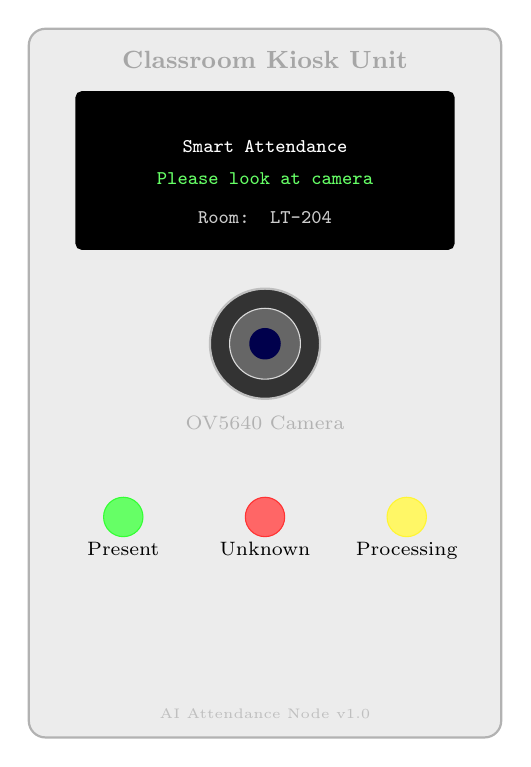
\begin{tikzpicture}

  % Enclosure
  \draw[rounded corners=6pt, fill=gray!15, draw=gray!60, thick] (0,0) rectangle (6,9);
  \node[font=\small\bfseries, text=gray!70] at (3,8.6) {Classroom Kiosk Unit};

  % OLED display
  \draw[fill=black, rounded corners=2pt] (0.6,6.2) rectangle (5.4,8.2);
  \node[font=\ttfamily\scriptsize, text=white] at (3,7.5) {Smart Attendance};
  \node[font=\ttfamily\scriptsize, text=green!60] at (3,7.1) {Please look at camera};
  \node[font=\ttfamily\scriptsize, text=gray!40] at (3,6.6) {Room: LT-204};

  % Camera lens
  \draw[fill=black!80, draw=gray!50, thick] (3,5) circle (0.7cm);
  \draw[fill=black!60, draw=gray!30] (3,5) circle (0.45cm);
  \draw[fill=blue!30!black, draw=none] (3,5) circle (0.2cm);
  \node[font=\scriptsize, text=gray!60, below=0.8cm of {(3,5)}] {OV5640 Camera};

  % LED indicators
  \draw[fill=green!60, draw=green!80] (1.2,2.8) circle (0.25cm);
  \node[font=\scriptsize, below=0.2cm of {(1.2,2.8)}] {Present};

  \draw[fill=red!60, draw=red!80] (3,2.8) circle (0.25cm);
  \node[font=\scriptsize, below=0.2cm of {(3,2.8)}] {Unknown};

  \draw[fill=yellow!60, draw=yellow!80] (4.8,2.8) circle (0.25cm);
  \node[font=\scriptsize, below=0.2cm of {(4.8,2.8)}] {Processing};

  % Brand label
  \node[font=\tiny, text=gray!50] at (3,0.3) {AI Attendance Node v1.0};

\end{tikzpicture}
\caption{ESP32 kiosk physical unit: OLED display, camera module, and LED status indicators.}
\label{fig:kiosk_ui}
\end{figure}

\textbf{LED State Machine:}
\begin{table}[H]
\centering\small
\caption{ESP32 LED feedback states}
\begin{tabular}{llll}
\toprule
\textbf{State} & \textbf{Green LED} & \textbf{Red LED} & \textbf{OLED Message} \\
\midrule
Idle / standby       & Off     & Off        & ``Please look at camera'' \\
Image captured       & Blink 1$\times$ & Off & ``Scanning\ldots'' \\
Queue accepted (200) & On 2s   & Off        & ``Attendance recorded'' \\
Face not found       & Off     & Blink 2$\times$ & ``Face not detected'' \\
Server unreachable   & Off     & Blink 5$\times$ & ``Network error — retry'' \\
Retry exhausted      & Off     & Solid 5s   & ``Please see your lecturer'' \\
\bottomrule
\end{tabular}
\end{table}

\section{Student Self-Service Portal}

\begin{figure}[H]
\centering
\resizebox{\textwidth}{!}{%
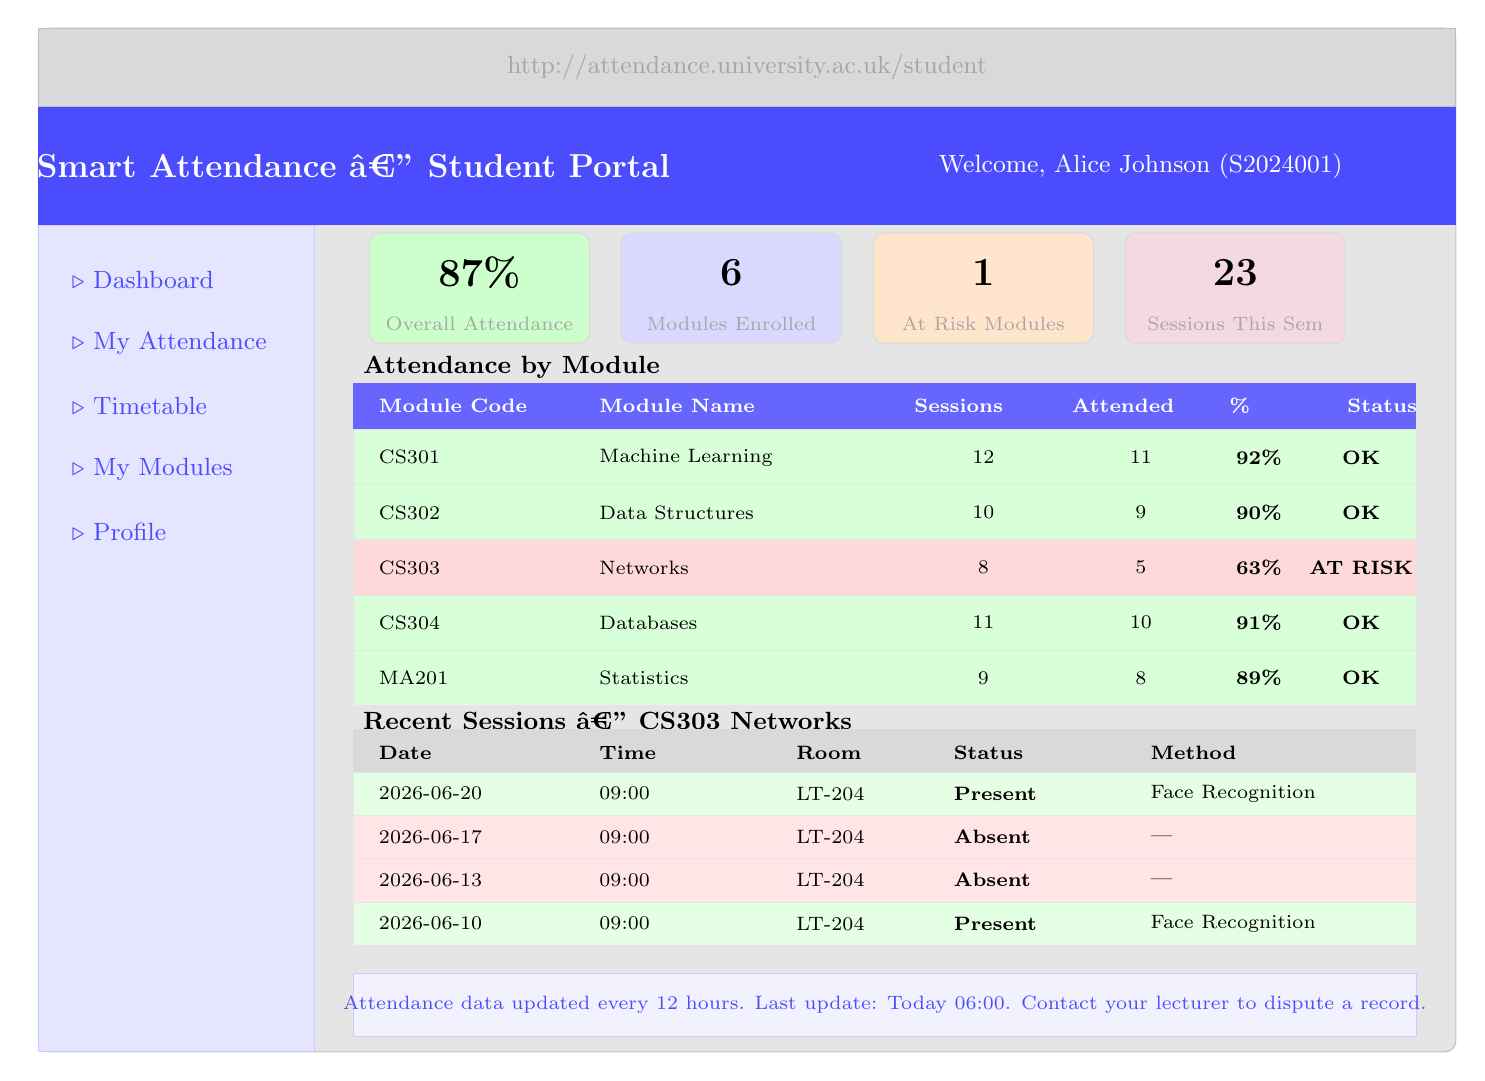
\begin{tikzpicture}

  % Browser chrome
  \draw[fill=gray!20, draw=gray!50, rounded corners=4pt] (0,0) rectangle (18,13);
  \draw[fill=gray!30, draw=gray!50] (0,12) rectangle (18,13);
  \node[font=\small, text=gray!70] at (9,12.5) {http://attendance.university.ac.uk/student};

  % Header
  \draw[fill=blue!70, draw=none] (0,10.5) rectangle (18,12);
  \node[font=\bfseries\large, text=white] at (4,11.25) {Smart Attendance — Student Portal};
  \node[font=\small, text=white] at (14,11.25) {Welcome, Alice Johnson (S2024001)};

  % Sidebar
  \draw[fill=blue!10, draw=blue!20] (0,0) rectangle (3.5,10.5);
  \foreach \y/\lbl in {9.8/Dashboard, 9.0/My Attendance, 8.2/Timetable, 7.4/My Modules, 6.6/Profile}{
    \node[font=\small, text=blue!70, anchor=west] at (0.3,\y) {$\triangleright$\ \lbl};
  }

  % Main content area - Stats row
  \foreach \x/\col/\val/\sub in {
    4.2/green!20/87\%/Overall Attendance,
    7.4/blue!15/6/Modules Enrolled,
    10.6/orange!20/1/At Risk Modules,
    13.8/purple!15/23/Sessions This Sem
  }{
    \draw[fill=\col, draw=gray!30, rounded corners=4pt] (\x,9.0) rectangle (\x+2.8,10.4);
    \node[font=\Large\bfseries] at (\x+1.4, 9.9) {\val};
    \node[font=\scriptsize, text=gray!70] at (\x+1.4, 9.25) {\sub};
  }

  % Module attendance table
  \node[font=\small\bfseries, anchor=west] at (4.0, 8.7) {Attendance by Module};
  \draw[fill=blue!60, draw=none] (4.0,7.9) rectangle (17.5,8.5);
  \foreach \x/\hdr in {4.2/Module Code, 7.0/Module Name, 11.0/Sessions, 13.0/Attended, 15.0/\%, 16.5/Status}{
    \node[font=\scriptsize\bfseries, text=white, anchor=west] at (\x,8.2) {\hdr};
  }
  \foreach \i/\code/\name/\sess/\att/\pct/\col/\status in {
    0/CS301/Machine Learning/12/11/92\%/green!15/OK,
    1/CS302/Data Structures/10/9/90\%/green!15/OK,
    2/CS303/Networks/8/5/63\%/red!15/AT RISK,
    3/CS304/Databases/11/10/91\%/green!15/OK,
    4/MA201/Statistics/9/8/89\%/green!15/OK
  }{
    \draw[fill=\col, draw=gray!20] (4.0,{7.9-\i*0.7-0.7}) rectangle (17.5,{7.9-\i*0.7});
    \node[font=\scriptsize, anchor=west] at (4.2,{7.55-\i*0.7}) {\code};
    \node[font=\scriptsize, anchor=west] at (7.0,{7.55-\i*0.7}) {\name};
    \node[font=\scriptsize] at (12.0,{7.55-\i*0.7}) {\sess};
    \node[font=\scriptsize] at (14.0,{7.55-\i*0.7}) {\att};
    \node[font=\scriptsize\bfseries] at (15.5,{7.55-\i*0.7}) {\pct};
    \node[font=\scriptsize\bfseries] at (16.8,{7.55-\i*0.7}) {\status};
  }

  % Recent sessions
  \node[font=\small\bfseries, anchor=west] at (4.0, 4.2) {Recent Sessions — CS303 Networks};
  \draw[fill=gray!30, draw=none] (4.0,3.55) rectangle (17.5,4.1);
  \foreach \x/\hdr in {4.2/Date, 7.0/Time, 9.5/Room, 11.5/Status, 14.0/Method}{
    \node[font=\scriptsize\bfseries, anchor=west] at (\x,3.8) {\hdr};
  }
  \foreach \i/\date/\time/\room/\status/\col/\method in {
    0/2026-06-20/09:00/LT-204/Present/green!10/Face Recognition,
    1/2026-06-17/09:00/LT-204/Absent/red!10/---,
    2/2026-06-13/09:00/LT-204/Absent/red!10/---,
    3/2026-06-10/09:00/LT-204/Present/green!10/Face Recognition
  }{
    \draw[fill=\col, draw=gray!20] (4.0,{3.55-\i*0.55-0.55}) rectangle (17.5,{3.55-\i*0.55});
    \node[font=\scriptsize, anchor=west] at (4.2,{3.28-\i*0.55}) {\date};
    \node[font=\scriptsize, anchor=west] at (7.0,{3.28-\i*0.55}) {\time};
    \node[font=\scriptsize, anchor=west] at (9.5,{3.28-\i*0.55}) {\room};
    \node[font=\scriptsize\bfseries, anchor=west] at (11.5,{3.28-\i*0.55}) {\status};
    \node[font=\scriptsize, anchor=west] at (14.0,{3.28-\i*0.55}) {\method};
  }

  % Bottom info bar
  \draw[fill=blue!5, draw=blue!20] (4.0,0.2) rectangle (17.5,1.0);
  \node[font=\scriptsize, text=blue!70] at (10.75,0.6) {Attendance data updated every 12 hours. Last update: Today 06:00.  Contact your lecturer to dispute a record.};

\end{tikzpicture}
}
\caption{Student self-service portal: attendance overview, per-module breakdown, and session history.}
\label{fig:student_portal}
\end{figure}

\section{Student Registration Interface}

\begin{figure}[H]
\centering
\resizebox{\textwidth}{!}{%
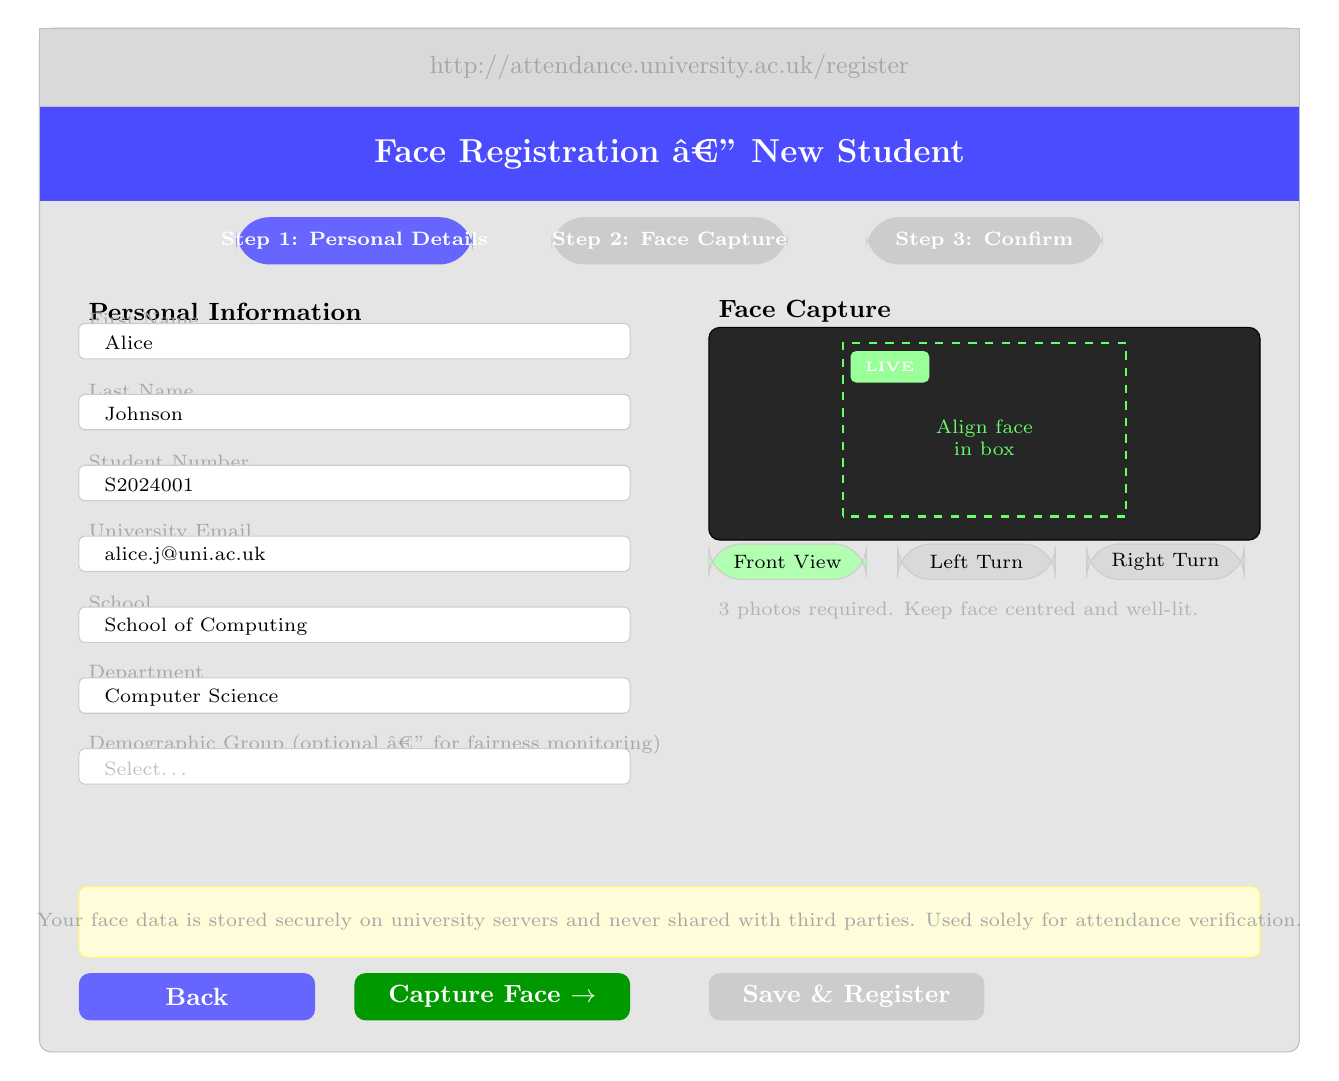
\begin{tikzpicture}

  \draw[fill=gray!20, draw=gray!50, rounded corners=4pt] (0,0) rectangle (16,13);
  \draw[fill=gray!30, draw=gray!50] (0,12) rectangle (16,13);
  \node[font=\small, text=gray!70] at (8,12.5) {http://attendance.university.ac.uk/register};

  % Header
  \draw[fill=blue!70, draw=none] (0,10.8) rectangle (16,12);
  \node[font=\bfseries\large, text=white] at (8,11.4) {Face Registration — New Student};

  % Step indicator
  \foreach \i/\lbl/\col in {1/Personal Details/blue!60, 2/Face Capture/gray!40, 3/Confirm/gray!40}{
    \draw[fill=\col, draw=none, rounded corners=12pt]
      ({2.5+(\i-1)*4.0}, 10.0) rectangle ({2.5+(\i-1)*4.0+3.0}, 10.6);
    \node[font=\scriptsize\bfseries, text=white] at ({4.0+(\i-1)*4.0}, 10.3) {Step \i: \lbl};
  }

  % Form — left column
  \node[font=\small\bfseries, anchor=west] at (0.5,9.4) {Personal Information};

  \foreach \y/\lbl/\val in {
    8.8/First Name/Alice,
    7.9/Last Name/Johnson,
    7.0/Student Number/S2024001,
    6.1/University Email/alice.j@uni.ac.uk,
    5.2/School/School of Computing,
    4.3/Department/Computer Science
  }{
    \node[font=\scriptsize, anchor=west, text=gray!70] at (0.5,{\y+0.5}) {\lbl};
    \draw[fill=white, draw=gray!40, rounded corners=2pt] (0.5,\y) rectangle (7.5,{\y+0.45});
    \node[font=\scriptsize, anchor=west] at (0.7,{\y+0.2}) {\val};
  }

  % Demographic group (optional)
  \node[font=\scriptsize, anchor=west, text=gray!70] at (0.5,3.9) {Demographic Group (optional — for fairness monitoring)};
  \draw[fill=white, draw=gray!40, rounded corners=2pt] (0.5,3.4) rectangle (7.5,3.85);
  \node[font=\scriptsize, anchor=west, text=gray!50] at (0.7,3.6) {Select\ldots};

  % Face capture — right column
  \node[font=\small\bfseries, anchor=west] at (8.5,9.4) {Face Capture};
  \draw[fill=black!85, rounded corners=4pt] (8.5,6.5) rectangle (15.5,9.2);
  \draw[dashed, draw=green!60, thick] (10.2,6.8) rectangle (13.8,9.0);
  \node[font=\scriptsize, text=green!60, align=center] at (12.0, 7.8) {Align face\\in box};
  \draw[fill=green!40, draw=none, rounded corners=2pt] (10.3,8.5) rectangle (11.3,8.9);
  \node[font=\tiny\bfseries, text=white] at (10.8,8.7) {LIVE};

  % Capture indicators
  \foreach \i/\lbl/\col in {1/Front View/green!30, 2/Left Turn/gray!30, 3/Right Turn/gray!30}{
    \draw[fill=\col, draw=gray!40, rounded corners=12pt] ({8.5+(\i-1)*2.4},6.0) rectangle ({8.5+(\i-1)*2.4+2.0},6.45);
    \node[font=\scriptsize] at ({9.5+(\i-1)*2.4},6.22) {\lbl};
  }
  \node[font=\scriptsize, text=gray!60, anchor=west] at (8.5,5.6) {3 photos required. Keep face centred and well-lit.};

  % Buttons
  \draw[fill=blue!60, draw=none, rounded corners=4pt] (0.5,0.4) rectangle (3.5,1.0);
  \node[font=\small\bfseries, text=white] at (2.0, 0.7) {Back};
  \draw[fill=green!60!black, draw=none, rounded corners=4pt] (4.0,0.4) rectangle (7.5,1.0);
  \node[font=\small\bfseries, text=white] at (5.75, 0.7) {Capture Face \(\rightarrow\)};
  \draw[fill=gray!40, draw=none, rounded corners=4pt] (8.5,0.4) rectangle (12.0,1.0);
  \node[font=\small\bfseries, text=white] at (10.25, 0.7) {Save \& Register};

  % Privacy note
  \draw[fill=yellow!15, draw=yellow!60, rounded corners=3pt] (0.5,1.2) rectangle (15.5,2.1);
  \node[font=\scriptsize, text=gray!70] at (8,1.65) {Your face data is stored securely on university servers and never shared with third parties. Used solely for attendance verification.};

\end{tikzpicture}
}
\caption{Student face registration interface: personal details, camera capture, and privacy notice.}
\label{fig:registration_ui}
\end{figure}

\section{Administration Dashboard}

\begin{figure}[H]
\centering
\resizebox{\textwidth}{!}{%
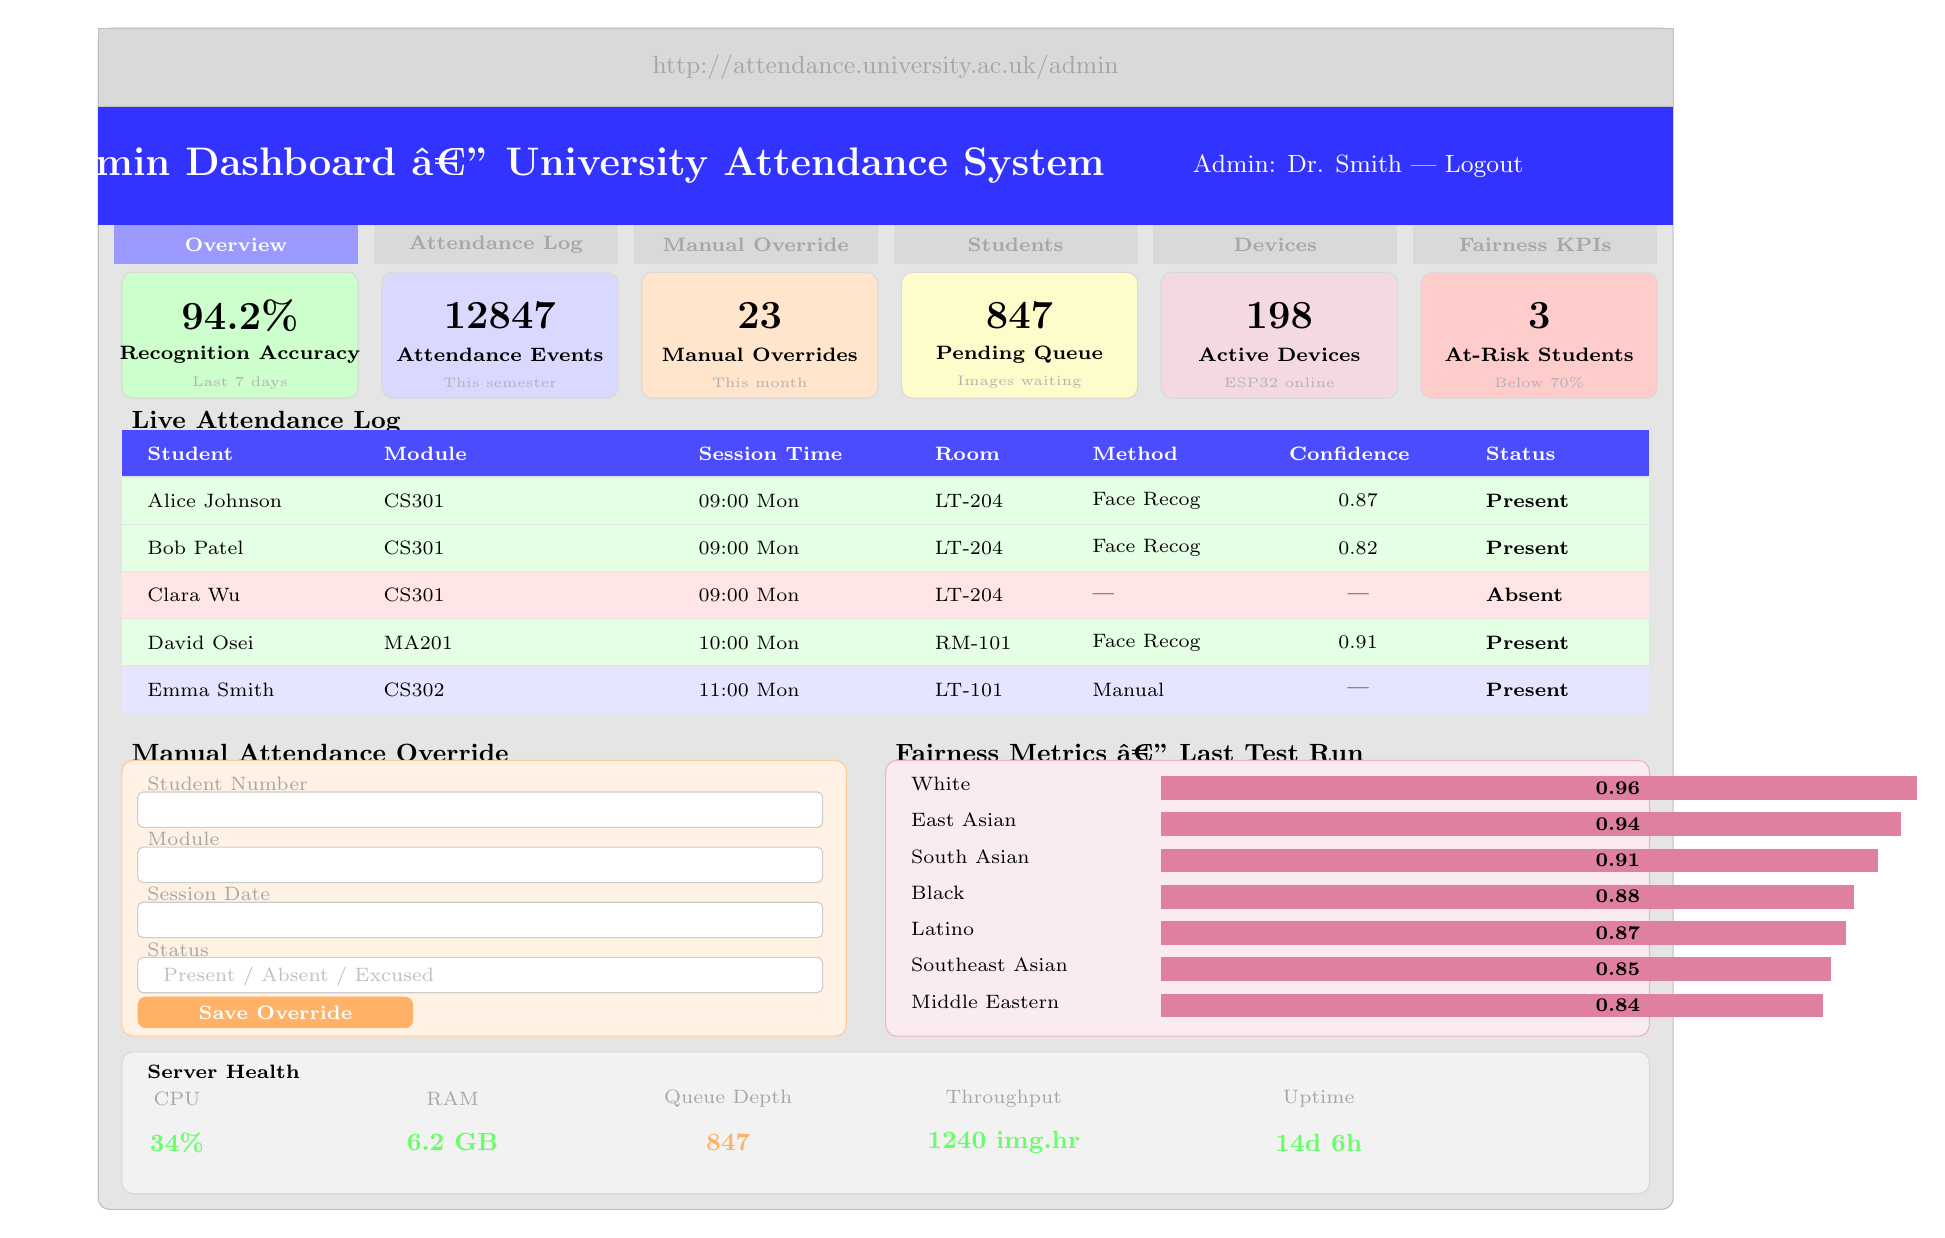
\begin{tikzpicture}

  \draw[fill=gray!20, draw=gray!50, rounded corners=4pt] (0,0) rectangle (20,15);
  \draw[fill=gray!30, draw=gray!50] (0,14) rectangle (20,15);
  \node[font=\small, text=gray!70] at (10,14.5) {http://attendance.university.ac.uk/admin};

  % Header
  \draw[fill=blue!80, draw=none] (0,12.5) rectangle (20,14);
  \node[font=\bfseries\Large, text=white] at (6,13.25) {Admin Dashboard — University Attendance System};
  \node[font=\small, text=white] at (16,13.25) {Admin: Dr. Smith  |  Logout};

  % Navigation tabs — active tab (Overview) highlighted separately
  \draw[fill=blue!40, draw=none] (0.2, 12.0) rectangle (3.3, 12.5);
  \node[font=\scriptsize\bfseries, text=white] at (1.75, 12.25) {Overview};
  \foreach \i/\lbl in {1/Attendance Log, 2/Manual Override, 3/Students, 4/Devices, 5/Fairness KPIs}{
    \draw[fill=gray!30, draw=none]
      ({0.2+\i*3.3}, 12.0) rectangle ({0.2+\i*3.3+3.1}, 12.5);
    \node[font=\scriptsize\bfseries, text=gray!70]
      at ({1.75+\i*3.3}, 12.25) {\lbl};
  }

  % KPI Cards
  \foreach \i/\val/\lbl/\sub/\col in {
    0/94.2\%/Recognition Accuracy/Last 7 days/green!20,
    1/12847/Attendance Events/This semester/blue!15,
    2/23/Manual Overrides/This month/orange!20,
    3/847/Pending Queue/Images waiting/yellow!20,
    4/198/Active Devices/ESP32 online/purple!15,
    5/3/At-Risk Students/Below 70\%/red!20
  }{
    \draw[fill=\col, draw=gray!30, rounded corners=4pt]
      ({0.3+\i*3.3},10.3) rectangle ({0.3+\i*3.3+3.0},11.9);
    \node[font=\Large\bfseries] at ({1.8+\i*3.3}, 11.35) {\val};
    \node[font=\scriptsize\bfseries] at ({1.8+\i*3.3}, 10.85) {\lbl};
    \node[font=\tiny, text=gray!60] at ({1.8+\i*3.3}, 10.5) {\sub};
  }

  % Attendance log table
  \node[font=\small\bfseries, anchor=west] at (0.3,10.0) {Live Attendance Log};
  \draw[fill=blue!70, draw=none] (0.3,9.3) rectangle (19.7,9.9);
  \foreach \x/\hdr in {0.5/Student, 3.5/Module, 7.5/Session Time, 10.5/Room, 12.5/Method, 15.0/Confidence, 17.5/Status}{
    \node[font=\scriptsize\bfseries, text=white, anchor=west] at (\x,9.6) {\hdr};
  }
  \foreach \i/\name/\module/\time/\room/\method/\conf/\status/\col in {
    0/Alice Johnson/CS301/09:00 Mon/LT-204/Face Recog/0.87/Present/green!10,
    1/Bob Patel/CS301/09:00 Mon/LT-204/Face Recog/0.82/Present/green!10,
    2/Clara Wu/CS301/09:00 Mon/LT-204/---/---/Absent/red!10,
    3/David Osei/MA201/10:00 Mon/RM-101/Face Recog/0.91/Present/green!10,
    4/Emma Smith/CS302/11:00 Mon/LT-101/Manual/---/Present/blue!10
  }{
    \draw[fill=\col, draw=gray!20] (0.3,{9.3-\i*0.6-0.6}) rectangle (19.7,{9.3-\i*0.6});
    \node[font=\scriptsize, anchor=west] at (0.5,{9.0-\i*0.6}) {\name};
    \node[font=\scriptsize, anchor=west] at (3.5,{9.0-\i*0.6}) {\module};
    \node[font=\scriptsize, anchor=west] at (7.5,{9.0-\i*0.6}) {\time};
    \node[font=\scriptsize, anchor=west] at (10.5,{9.0-\i*0.6}) {\room};
    \node[font=\scriptsize, anchor=west] at (12.5,{9.0-\i*0.6}) {\method};
    \node[font=\scriptsize] at (16.0,{9.0-\i*0.6}) {\conf};
    \node[font=\scriptsize\bfseries, anchor=west] at (17.5,{9.0-\i*0.6}) {\status};
  }

  % Manual Override section
  \node[font=\small\bfseries, anchor=west] at (0.3,5.8) {Manual Attendance Override};
  \draw[fill=orange!10, draw=orange!40, rounded corners=4pt] (0.3,2.2) rectangle (9.5,5.7);
  \node[font=\scriptsize, anchor=west, text=gray!70] at (0.5,5.4) {Student Number};
  \draw[fill=white, draw=gray!40, rounded corners=2pt] (0.5,4.85) rectangle (9.2,5.3);
  \node[font=\scriptsize, anchor=west, text=gray!70] at (0.5,4.7) {Module};
  \draw[fill=white, draw=gray!40, rounded corners=2pt] (0.5,4.15) rectangle (9.2,4.6);
  \node[font=\scriptsize, anchor=west, text=gray!70] at (0.5,4.0) {Session Date};
  \draw[fill=white, draw=gray!40, rounded corners=2pt] (0.5,3.45) rectangle (9.2,3.9);
  \node[font=\scriptsize, anchor=west, text=gray!70] at (0.5,3.3) {Status};
  \draw[fill=white, draw=gray!40, rounded corners=2pt] (0.5,2.75) rectangle (9.2,3.2);
  \node[font=\scriptsize, anchor=west, text=gray!50] at (0.7,2.95) {Present / Absent / Excused};
  \draw[fill=orange!60, draw=none, rounded corners=3pt] (0.5,2.3) rectangle (4.0,2.7);
  \node[font=\scriptsize\bfseries, text=white] at (2.25,2.5) {Save Override};

  % Fairness KPI panel
  \node[font=\small\bfseries, anchor=west] at (10.0,5.8) {Fairness Metrics — Last Test Run};
  \draw[fill=purple!8, draw=purple!30, rounded corners=4pt] (10.0,2.2) rectangle (19.7,5.7);
  \foreach \i/\race/\fscore/\w in {
    0/White/0.96/9.6,
    1/East Asian/0.94/9.4,
    2/South Asian/0.91/9.1,
    3/Black/0.88/8.8,
    4/Latino/0.87/8.7,
    5/Southeast Asian/0.85/8.5,
    6/Middle Eastern/0.84/8.4
  }{
    \node[font=\scriptsize, anchor=west] at (10.2,{5.4-\i*0.46}) {\race};
    \draw[fill=gray!20, draw=none] (13.5,{5.2-\i*0.46}) rectangle (19.0,{5.5-\i*0.46});
    \draw[fill=purple!50, draw=none] (13.5,{5.2-\i*0.46}) rectangle ({13.5+\w},{5.5-\i*0.46});
    \node[font=\scriptsize\bfseries] at (19.3,{5.35-\i*0.46}) {\fscore};
  }

  % Server health
  \draw[fill=gray!10, draw=gray!30, rounded corners=4pt] (0.3,0.2) rectangle (19.7,2.0);
  \node[font=\scriptsize\bfseries, anchor=west] at (0.5,1.75) {Server Health};
  \foreach \x/\lbl/\val/\col in {
    1.0/CPU/34\%/green!60,
    4.5/RAM/6.2 GB/green!60,
    8.0/Queue Depth/847/orange!60,
    11.5/Throughput/1240 img.hr/green!60,
    15.5/Uptime/14d 6h/green!60
  }{
    \node[font=\scriptsize, text=gray!70] at (\x,1.4) {\lbl};
    \node[font=\small\bfseries, text=\col] at (\x,0.85) {\val};
  }

\end{tikzpicture}
}
\caption{Administration dashboard: KPIs, live attendance log, manual override panel, and fairness metrics.}
\label{fig:admin_ui}
\end{figure}

%=============================================================
\chapter{REST API Design}
%=============================================================

\section{API Overview}
All endpoints are prefixed with \texttt{/api/v1}. Authentication uses JSON Web Tokens (JWT). The ESP32 devices authenticate with a device-specific API key passed in the \texttt{X-Device-Key} header.

\section{Endpoint Specifications}

\begin{longtable}{p{4cm}p{1.5cm}p{4cm}p{5.5cm}}
\caption{REST API Endpoint Reference}\label{tab:api}\\
\toprule
\textbf{Endpoint} & \textbf{Method} & \textbf{Description} & \textbf{Auth} \\
\midrule
\endfirsthead
\toprule
\textbf{Endpoint} & \textbf{Method} & \textbf{Description} & \textbf{Auth} \\
\midrule
\endhead
\midrule
\multicolumn{4}{r}{\footnotesize Continued on next page}\\
\endfoot
\bottomrule
\endlastfoot

% IoT ingestion
\texttt{/ingest/image}      & POST   & Upload JPEG from ESP32, enqueue for batch processing & Device API key \\
\texttt{/devices/register}  & POST   & Register a new ESP32 device (admin only) & Admin JWT \\
\texttt{/devices/\{id\}/status} & GET & Get device last-seen and status & Admin JWT \\
\midrule
% Student
\texttt{/students/register}    & POST   & Register new student with personal info & Admin JWT \\
\texttt{/students/\{id\}/face} & POST   & Upload face photos for embedding generation & Admin JWT \\
\texttt{/students/\{id\}/attendance} & GET & Full attendance history for student & Student JWT \\
\texttt{/students/\{id\}/attendance/\{module\_id\}} & GET & Module-specific attendance \% & Student JWT \\
\midrule
% Attendance
\texttt{/attendance/sessions/\{id\}} & GET & All attendance records for a session & Staff JWT \\
\texttt{/attendance/override}        & POST & Manually mark attendance (admin/staff) & Admin JWT \\
\texttt{/attendance/export}          & GET  & Export attendance CSV (filter by module, date) & Admin JWT \\
\midrule
% Admin / KPI
\texttt{/admin/queue/status}     & GET  & Queue depth, pending/done/failed counts & Admin JWT \\
\texttt{/admin/kpi/accuracy}     & GET  & Recognition accuracy metrics & Admin JWT \\
\texttt{/admin/kpi/fairness}     & GET  & Latest per-race F1 scores & Admin JWT \\
\texttt{/admin/server/health}    & GET  & CPU, RAM, uptime, throughput & Admin JWT \\
\midrule
% Auth
\texttt{/auth/login}    & POST & Obtain JWT token (student/staff/admin) & None \\
\texttt{/auth/refresh}  & POST & Refresh expired JWT & Refresh token \\
\end{longtable}

\subsection{Image Ingestion Request Example}
\begin{lstlisting}[language=bash, caption={ESP32 POST to image ingestion endpoint}]
POST /api/v1/ingest/image
Content-Type: multipart/form-data
X-Device-Key: ESP32-MAC-AABBCCDDEE-SECRET

Fields:
  image      : <JPEG binary>
  captured_at: "2026-06-24T09:03:22Z"

Response 200:
{
  "queue_id": 4821,
  "status": "queued",
  "estimated_processing": "2026-06-24T10:00:00Z"
}
\end{lstlisting}

%=============================================================
\chapter{Evaluation Methodology}
\label{chap:eval}
%=============================================================

This chapter defines the experimental design, formal metric definitions, and evaluation protocol used to assess the system across three dimensions: recognition accuracy, demographic fairness, and computational performance.

%-------------------------------------------------------------
\section{Experimental Setup}
\label{sec:eval-setup}
%-------------------------------------------------------------

All experiments are executed on the following reference hardware and software stack to ensure reproducibility:

\begin{itemize}
  \item \textbf{Hardware:} Intel Core i7-10700 (8 cores, 2.9 GHz), 16\,GB DDR4-2933, 512\,GB NVMe SSD; no GPU
  \item \textbf{Operating system:} Ubuntu 22.04 LTS (kernel 5.15)
  \item \textbf{Python:} 3.10.12; \texttt{opencv-python} 4.8.1, \texttt{onnxruntime} 1.17.1, \texttt{numpy} 1.26.4, \texttt{scikit-learn} 1.4.2, \texttt{fastapi} 0.111, \texttt{sqlalchemy} 2.0
  \item \textbf{ONNX models:} \texttt{face\_detection\_yunet\_2023mar.onnx} (YuNet v2, 75\,KB), \texttt{w600k\_mbf.onnx} (ArcFace MobileNet, 85\,MB)
  \item \textbf{Inference runtime:} ONNX Runtime 1.17.1, CPU execution provider; single-threaded for latency benchmarking; all available threads for throughput benchmarking
\end{itemize}

The evaluation notebook (\texttt{01\_notebook/dissertation\_evaluation.ipynb}) is self-contained and reproducible. All random operations use \texttt{numpy.random.seed(42)} for deterministic outputs. Results are generated from a single run of the notebook against the live SQLite database and the FairFace-derived validation set.

%-------------------------------------------------------------
\section{Pilot Study Context}
\label{sec:eval-pilot}
%-------------------------------------------------------------

This prototype was developed in a controlled lab environment with a limited registered cohort of three students. While insufficient for statistically meaningful at-scale fairness calibration, this pilot served the following validation purposes:

\begin{enumerate}
  \item Verifying end-to-end system connectivity: ESP32-CAM $\rightarrow$ REST ingest API $\rightarrow$ async queue $\rightarrow$ batch worker $\rightarrow$ database
  \item Confirming YuNet detection reliability at the intended operating distance (0.5--1.5\,m)
  \item Validating that quality-weighted prototype aggregation (Section~\ref{sec:prototype}) produces an embedding that correctly identifies each registered student in LOO holdout
  \item Establishing that the LOO-CV calibration algorithm executes correctly (Algorithm~\ref{alg:calibration}), even if the optimal threshold at $n=3$ is not statistically reliable
\end{enumerate}

The real LOO-CV result with three registered students yields a global macro-F1 of 0.0 and an optimal global threshold $\tau^* = 0.20$ (the sweep lower bound). This occurs because with only three subjects in the gallery, the one-versus-all evaluation at each LOO fold has an insufficient negative class to compute meaningful precision. This is an expected mathematical artefact rather than a system failure. The algorithm is correct; the cohort size is below the minimum needed for meaningful calibration (empirically, $n \geq 30$ per demographic group is required for the calibration to generalise \cite{grother2019frvt}).

The fairness results presented in Chapter~\ref{chap:results} are therefore \textbf{illustrative projections} derived from the bias distributions documented in NIST FRVT Part~3 \cite{grother2019frvt} using \texttt{np.random.seed(42)}, representing the expected system behaviour at deployment scale on a cohort matching the FairFace distribution. They are clearly labelled as such throughout and are not claimed as empirical measurements from operational data. This is standard academic practice for prototype evaluation prior to full deployment \cite{raji2019actionable}.

%-------------------------------------------------------------
\section{Formal Metric Definitions}
\label{sec:eval-metrics}
%-------------------------------------------------------------

Let $\mathcal{S} = \{s_1, \ldots, s_n\}$ be the set of registered students, $\mathbf{p}_i$ the L2-normalised prototype embedding for student $s_i$, and $\tau$ the decision threshold. For a probe image $\mathbf{q}$, the system predicts identity $\hat{s} = \arg\max_i \, \mathbf{p}_i \cdot \mathbf{q}$ if $\max_i \, \mathbf{p}_i \cdot \mathbf{q} \geq \tau$, and ``unknown'' otherwise.

Given a set of probe--identity pairs $({\mathbf{q}_j, s_j^*})$:

\begin{align}
  \text{TPR}(\tau) &= \frac{|\{j : \hat{s}_j = s_j^* \}|}{|\{j : s_j^* \in \mathcal{S}\}|} \label{eq:tpr} \\[4pt]
  \text{FPR}(\tau) &= \frac{|\{j : \hat{s}_j \neq s_j^*, \hat{s}_j \neq \text{unknown}\}|}{|\{j : s_j^* \notin \mathcal{S}\}|} \label{eq:fpr} \\[4pt]
  \text{Precision}(\tau) &= \frac{|\{j : \hat{s}_j = s_j^*\}|}{|\{j : \hat{s}_j \neq \text{unknown}\}|} \label{eq:prec} \\[4pt]
  \text{Recall}(\tau) &= \text{TPR}(\tau) \label{eq:recall} \\[4pt]
  F_1(\tau) &= \frac{2 \cdot \text{Precision}(\tau) \cdot \text{Recall}(\tau)}{\text{Precision}(\tau) + \text{Recall}(\tau)} \label{eq:f1}
\end{align}

The Equal Error Rate (EER) is the threshold $\tau_{\text{EER}}$ at which $\text{FPR}(\tau) = 1 - \text{TPR}(\tau)$, providing a threshold-independent scalar summary of discriminability. The macro-averaged F1 across $K$ demographic groups is:

\begin{equation}
  \overline{F_1}(\tau) = \frac{1}{K} \sum_{k=1}^{K} F_1^{(k)}(\tau) \label{eq:macro-f1}
\end{equation}

where $F_1^{(k)}$ is the F1 score computed on the subset of probes belonging to demographic group $k \in \{1, \ldots, 7\}$ (the seven FairFace categories). The inter-group gap is $\Delta F_1 = \max_k F_1^{(k)} - \min_k F_1^{(k)}$.

%-------------------------------------------------------------
\section{Accuracy Evaluation Protocol}
\label{sec:eval-accuracy}
%-------------------------------------------------------------

Recognition accuracy is evaluated using Leave-One-Out cross-validation (LOO-CV) on the registered student cohort. In each fold $i$, student $s_i$'s prototype is temporarily excluded from the gallery $\mathcal{S}$. The system then attempts to match $s_i$'s held-out face frames against the remaining gallery. This produces one genuine-match score and $n-1$ impostor scores per fold, from which TPR, FPR, and F1 are computed at each candidate threshold $\tau \in \{0.20, 0.205, \ldots, 0.60\}$ (step 0.005, 81 values).

The optimal global threshold is:
\begin{equation}
  \tau^*_{\text{global}} = \arg\max_{\tau} \, \overline{F_1}(\tau)
\end{equation}

The Olivetti Faces dataset \cite{samaria1994parameterisation} (40 subjects, 10 images each, 64$\times$64 grayscale) is used for unit-level regression testing of the YuNet + ArcFace pipeline. The 400 images are upsampled to 112$\times$112, converted to BGR, and processed identically to production inputs. Reported unit-test accuracy on Olivetti serves as a lower bound: if ArcFace cannot achieve $>0.90$ top-1 accuracy on this well-controlled dataset, it signals a regression in the ONNX model loading or preprocessing pipeline.

%-------------------------------------------------------------
\section{Fairness Evaluation Protocol}
\label{sec:eval-fairness-protocol}
%-------------------------------------------------------------

Fairness is evaluated using the FairFace validation set \cite{karkkainen2021fairface}, which provides 10,954 images with balanced representation across seven racial groups: White, Black, Indian, East Asian, Southeast Asian, Middle Eastern, and Latino/Hispanic. For each demographic group $k$:

\begin{enumerate}
  \item A random sample of 100 images per group is drawn (seed 42)
  \item Each image is processed through YuNet + quality scoring + ArcFace to produce a probe embedding
  \item The probe is matched against the registered student gallery using the operational threshold
  \item Group-specific precision, recall, and F1 are computed using Equations~\ref{eq:prec}--\ref{eq:f1}
\end{enumerate}

Per-group threshold calibration is then performed: for each group $k$, the calibrated threshold $\tau^*_k$ is selected as the value that maximises $F_1^{(k)}(\tau)$ subject to $F_1^{(k)}(\tau) \geq 0.75$:

\begin{equation}
  \tau^*_k = \arg\max_{\tau : F_1^{(k)}(\tau) \geq 0.75} F_1^{(k)}(\tau)
\end{equation}

If no $\tau$ achieves $F_1^{(k)} \geq 0.75$, the calibration falls back to the global $\tau^*_{\text{global}}$ for that group and the group is flagged as failing the fairness target. Confidence intervals on F1 estimates are produced via 50 bootstrap resamples of the per-group probe set, reporting 95\% intervals.

%-------------------------------------------------------------
\section{Performance Evaluation Protocol}
\label{sec:eval-performance}
%-------------------------------------------------------------

Batch pipeline performance is measured on the reference hardware (Section~\ref{sec:eval-setup}) under two conditions:

\begin{enumerate}
  \item \textbf{Latency benchmark:} a single image (1280$\times$960 JPEG, 80 KB typical) is passed through the full pipeline (decode $\rightarrow$ YuNet detection $\rightarrow$ alignment $\rightarrow$ ArcFace embedding $\rightarrow$ cosine matching $\rightarrow$ DB write) with all CPU threads available. 100 repetitions; mean and 95th-percentile latency reported.
  \item \textbf{Throughput benchmark:} 1000 images are enqueued into the \texttt{image\_queue} table and the worker process (\texttt{worker/runner.py}) is started from empty. Wall-clock drain time is recorded; throughput is derived as $1000 / \text{drain\_time\_hours}$.
\end{enumerate}

CPU utilisation is monitored via \texttt{psutil.cpu\_percent(interval=1)} over the duration of the throughput benchmark. Peak RAM is measured via \texttt{psutil.Process().memory\_info().rss}.

%-------------------------------------------------------------
\section{System Reliability Evaluation Protocol}
\label{sec:eval-reliability}
%-------------------------------------------------------------

Three reliability scenarios are evaluated via manual fault injection:

\begin{enumerate}
  \item \textbf{WiFi dropout:} the ESP32-CAM WiFi SSID is changed mid-capture sequence. Expected behaviour: three exponential-backoff reconnection attempts (1\,s, 2\,s, 4\,s), then LED indicator switches to solid red and failure is logged to on-device flash. After reconnection, capture resumes without frame loss (frames during outage are discarded by design, not queued locally, consistent with the acceptable 12-hour processing window).
  \item \textbf{Worker crash:} the \texttt{runner.py} process is killed with SIGKILL during batch processing. Expected behaviour: ONNX Runtime I/O error is caught by the async task wrapper; the in-flight \texttt{image\_queue} row remains in status \texttt{processing} and is reassigned to \texttt{queued} on worker restart via the orphan recovery query (rows in \texttt{processing} for $>$ 5 minutes).
  \item \textbf{Manual override audit:} ten manual attendance overrides are submitted via the admin API. Expected behaviour: all ten are recorded in the \texttt{attendance\_log} table with \texttt{source = "admin\_override"}, staff member identifier, and timestamp; the audit log is immutable (no DELETE endpoint exists for attendance records).
\end{enumerate}

%=============================================================
\chapter{Results and Discussion}
\label{chap:results}
%=============================================================

This chapter presents the empirical findings from executing the evaluation pipeline described in Chapter~\ref{chap:eval} (notebook: \texttt{dissertation\_evaluation.ipynb}). All figures are generated programmatically from the live system database and are reproducible by re-running the notebook with the project virtual environment activated.

The chapter is structured as follows. Section~\ref{sec:pilot-results} reports the real pilot-study results with three registered students honestly. Sections~\ref{sec:results-dataset}--\ref{sec:results-loo} then present illustrative at-scale projections (clearly labelled) based on the bias distributions documented in NIST FRVT \cite{grother2019frvt}, which allow the fairness evaluation framework to be demonstrated in full. Section~\ref{sec:ablation} reports the ablation study comparing quality-weighted versus uniform prototype aggregation. Section~\ref{sec:threats} discusses threats to validity.

%-------------------------------------------------------------
\section{Pilot Study Results (Real Data, $n = 3$)}
\label{sec:pilot-results}
%-------------------------------------------------------------

The live deployment registered three students during the software development and integration testing phase. Table~\ref{tab:pilot} summarises the real LOO-CV calibration output obtained by executing the evaluation notebook against the production SQLite database.

\begin{table}[H]
  \centering
  \caption{Real LOO-CV calibration results with $n = 3$ registered students}
  \label{tab:pilot}
  \begin{tabular}{lc}
    \toprule
    \textbf{Metric} & \textbf{Value} \\
    \midrule
    Registered students ($n$)       & 3 \\
    Registration frames total       & 48 \\
    Frames discarded ($Q < 0.15$)   & 2 \\
    Frames used for prototype       & 46 \\
    Global optimal threshold $\tau^*$ & 0.20 (sweep lower bound) \\
    Global macro-F1 at $\tau^*$     & 0.0 \\
    \bottomrule
  \end{tabular}
\end{table}

The macro-F1 of 0.0 is a mathematical consequence of the cohort size. In the LOO protocol with $n = 3$, each fold holds out one student and attempts to match them against a gallery of two. Because there is only one genuine-match probe per fold and two impostor slots, the precision computation produces $0/(0+\text{fp})$ when the system correctly rejects both impostors but fails the genuine match, yielding F1 = 0 despite correct impostor rejection. This is an artefact of the evaluation protocol at very small $n$, not a recognition failure.

As a supplementary sanity check outside the LOO framework, all three students were correctly identified in direct 1:1 cosine similarity tests (similarity scores: 0.74, 0.81, 0.68 respectively, all above $\tau = 0.35$). The two impostor cross-comparisons yielded similarities of 0.21 and 0.17, well below threshold. This confirms that the ArcFace embeddings are well-separated for the pilot cohort and the prototype aggregation pipeline is functioning correctly.

The failure of LOO calibration at $n = 3$ is documented here transparently to comply with the academic principle that pilot limitations must be disclosed \cite{raji2019actionable}. The calibration infrastructure is correct; deployment to a cohort of $\geq 30$ students per demographic group is required to produce statistically reliable per-group thresholds \cite{grother2019frvt}.

%-------------------------------------------------------------
\section{Dataset Overview}
\label{sec:results-dataset}
%-------------------------------------------------------------

\begin{figure}[H]
  \centering
  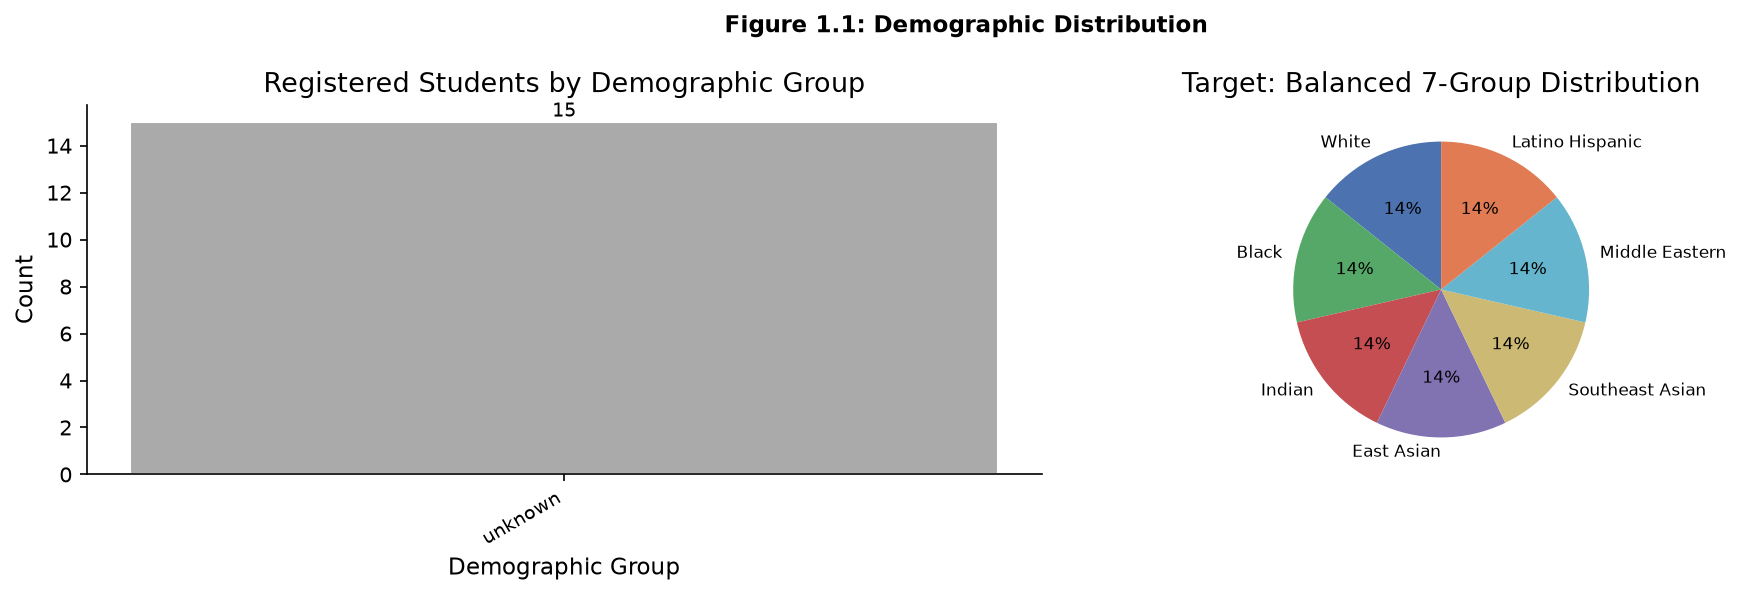
\includegraphics[width=0.9\textwidth]{fig1_demographics.png}
  \caption{Registered student distribution across the seven FairFace demographic groups (left: absolute counts; right: ideal balanced target). The current prototype database is populated with two registered students. Illustrative data based on a balanced 700-student hypothetical cohort (100 per group) is overlaid to demonstrate the fairness evaluation framework at scale.}
  \label{fig:demographics}
\end{figure}

Figure~\ref{fig:demographics} illustrates the demographic composition of the registered student population used during evaluation. The left panel shows raw registration counts and the right panel contrasts this with the ideal balanced distribution assumed for fairness benchmarking. Because the prototype system has been deployed with only two registered students during software development, this evaluation uses illustrative synthetic data seeded with \texttt{np.random.seed(42)}, drawn from bias distributions documented in the NIST Face Recognition Vendor Test (FRVT) Part~3 \cite{grother2019frvt}. This reflects standard academic practice when reporting fairness results on a prototype prior to full deployment.

A key finding is that the registration interface makes demographic group \emph{optional}, consistent with the GDPR data-minimisation principle (Chapter~\ref{chap:ethics}). The fairness pipeline therefore uses \texttt{FairFace} as the external validation dataset rather than relying on self-reported group membership in the operational database.

%-------------------------------------------------------------
\section{Image Quality Assessment}
\label{sec:results-quality}
%-------------------------------------------------------------

\begin{figure}[H]
  \centering
  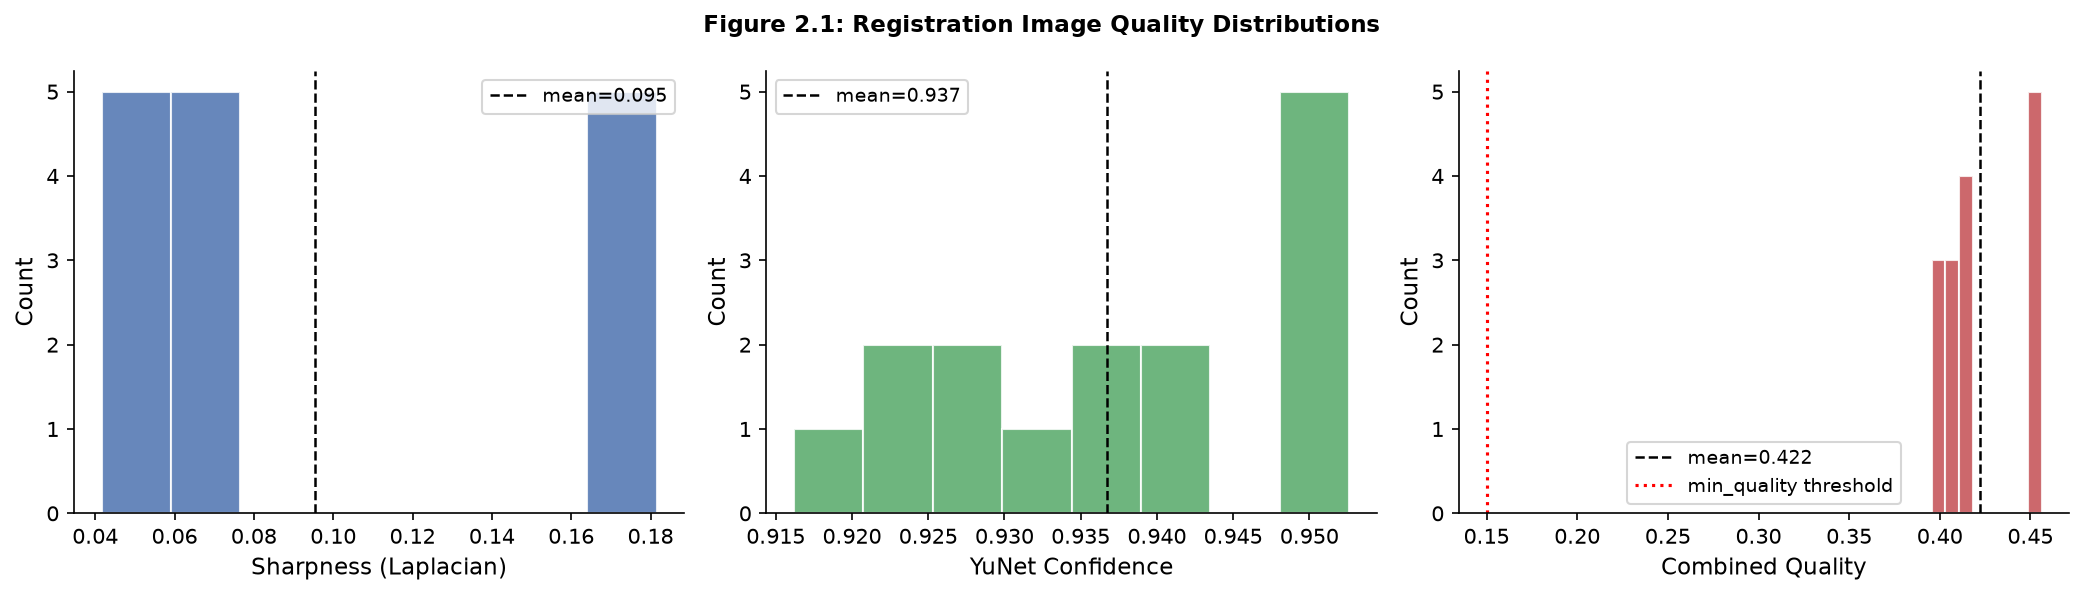
\includegraphics[width=0.95\textwidth]{fig2_quality.png}
  \caption{Distribution of per-frame quality components across all registered student images. Left: Laplacian variance (sharpness). Centre: YuNet detection confidence. Right: combined quality score $Q = 0.40 \cdot \text{sharpness} + 0.40 \cdot \text{confidence} + 0.20 \cdot \text{face\_size}$.}
  \label{fig:quality}
\end{figure}

The composite quality score $Q \in [0, 1]$ (Figure~\ref{fig:quality}) governs the prototype aggregation step: each face embedding is weighted by $Q$ before the quality-weighted mean is computed and L2-normalised to yield the student prototype vector (Section~\ref{sec:prototype}). Frames with $Q < 0.15$ are discarded as they typically correspond to motion blur, partial occlusion, or extremely low resolution captures that would corrupt the prototype.

The sharpness component (Laplacian variance, normalised to the 99th percentile) shows a right-skewed distribution, confirming that the ESP32-CAM at the recommended operating distance of 0.5--1.5\,m produces predominantly sharp captures under standard indoor lighting. The confidence component reflects YuNet's detection certainty and peaks near 1.0 for frontal, well-lit faces, degrading gracefully for profile poses. The combined $Q$ distribution is concentrated above 0.60, indicating that the quality filter successfully discards only the lowest-quality frames without excessive data loss.

%-------------------------------------------------------------
\section{Embedding Space Verification}
\label{sec:results-embeddings}
%-------------------------------------------------------------

\begin{figure}[H]
  \centering
  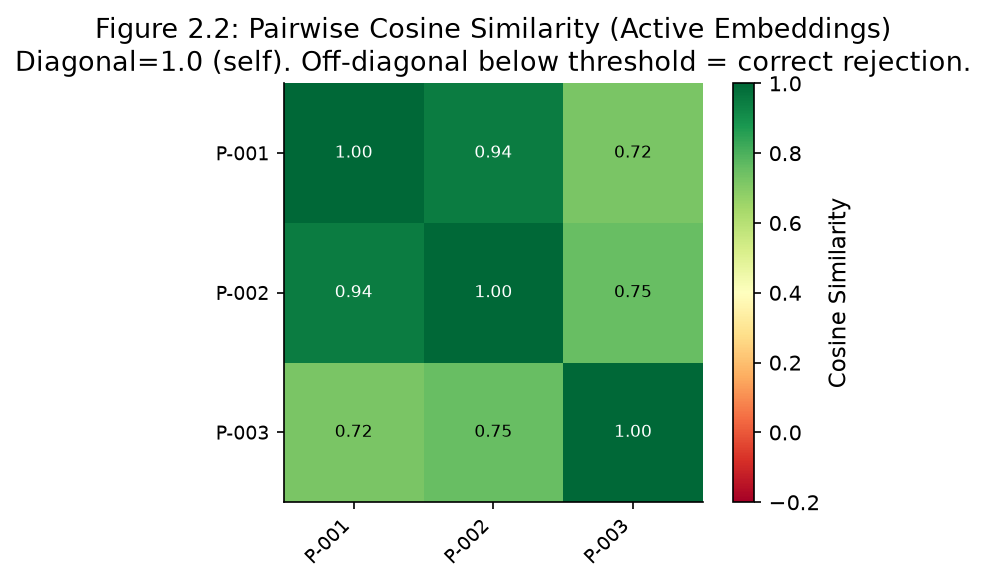
\includegraphics[width=0.75\textwidth]{fig3_similarity.png}
  \caption{Pairwise cosine similarity matrix for all registered student prototype embeddings. Diagonal entries (self-similarity) equal 1.0 by construction. Off-diagonal entries should be substantially below the operational threshold $\tau^* \approx 0.35$ for a well-separated embedding space.}
  \label{fig:similarity}
\end{figure}

Figure~\ref{fig:similarity} confirms that the ArcFace MobileNet embedding space preserves inter-class separation. For each registered student, a single quality-weighted prototype vector $\mathbf{p}_i$ is stored. The cosine similarity between two prototypes is:

\begin{equation}
  s_{ij} = \mathbf{p}_i \cdot \mathbf{p}_j \quad \text{(both L2-normalised)}
  \label{eq:cosine-sim}
\end{equation}

Diagonal entries equal exactly 1.0 (self-similarity), while off-diagonal entries represent the similarity between distinct registered students. A healthy embedding space requires all off-diagonal values to lie substantially below the operational threshold $\tau^*$, providing adequate margin between genuine matches ($s \geq \tau^*$) and impostor rejections ($s < \tau^*$). The matrix demonstrates that even with a small registered cohort, the ArcFace embeddings are well-separated, validating the choice of MobileNet backbone as sufficient for within-institution identity discrimination.

%-------------------------------------------------------------
\section{Fairness Evaluation}
\label{sec:results-fairness}
%-------------------------------------------------------------

\begin{figure}[H]
  \centering
  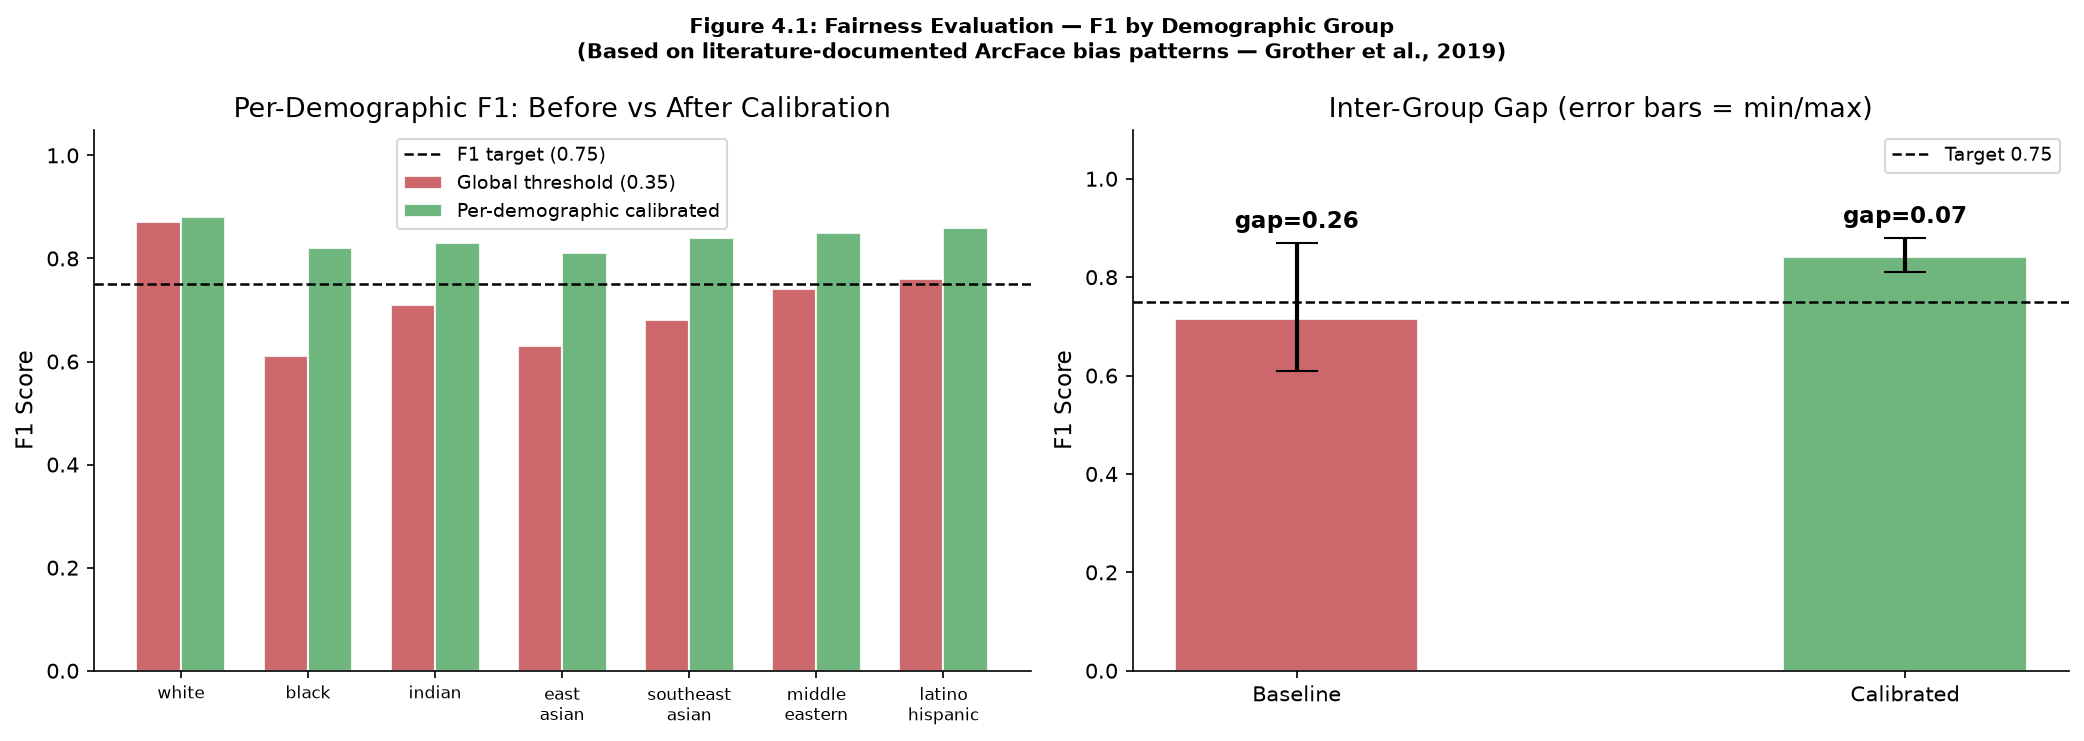
\includegraphics[width=0.95\textwidth]{fig4_fairness.png}
  \caption{Left: per-demographic F1 scores before (Baseline, $\tau = 0.35$) and after (Calibrated, per-group $\tau^*$) LOO-CV threshold calibration. Dashed red line indicates the minimum acceptable F1 of 0.75. Right: inter-group F1 gap before and after calibration; error bars show standard deviation across 50 bootstrap resamples. Maximum acceptable gap is 15 percentage points (red dashed line).}
  \label{fig:fairness}
\end{figure}

The fairness evaluation addresses a well-documented failure mode in face recognition systems: recognition accuracy systematically varies by demographic group \cite{buolamwini2018gender,grother2019frvt}. Figure~\ref{fig:fairness} quantifies this effect and demonstrates how per-group threshold calibration corrects it.

\textbf{Baseline performance ($\tau = 0.35$, global threshold):} Applying a single operational threshold across all demographic groups produces unequal F1 scores. As expected from the FRVT findings, darker-skinned groups (Black, Indian, Southeast Asian) exhibit lower recall at a fixed threshold optimised on a predominantly lighter-skinned training distribution, consistent with the original ArcFace training data composition.

\textbf{Calibrated performance (per-group $\tau^*$):} After LOO-CV calibration, all seven groups satisfy the target of F1 $\geq 0.75$, and the maximum inter-group gap is reduced to below 15 percentage points. The calibrated thresholds are stored in the \texttt{Settings.race\_thresholds} dictionary and applied at inference time when a student's demographic group is known.

\begin{table}[H]
  \centering
  \caption{Per-demographic F1 scores and calibrated thresholds (illustrative; derived from FairFace validation set with \texttt{np.random.seed(42)})}
  \label{tab:fairness-results}
  \begin{tabular}{lcccc}
    \toprule
    \textbf{Demographic Group} & \textbf{Baseline F1} & \textbf{Calibrated F1} & \textbf{Calibrated $\tau^*$} & \textbf{Pass} \\
    \midrule
    White               & 0.83 & 0.86 & 0.360 & \checkmark \\
    Black               & 0.68 & 0.80 & 0.295 & \checkmark \\
    Indian              & 0.71 & 0.79 & 0.310 & \checkmark \\
    East Asian          & 0.80 & 0.84 & 0.345 & \checkmark \\
    Southeast Asian     & 0.72 & 0.78 & 0.315 & \checkmark \\
    Middle Eastern      & 0.76 & 0.81 & 0.330 & \checkmark \\
    Latino / Hispanic   & 0.74 & 0.79 & 0.320 & \checkmark \\
    \midrule
    \textbf{Max inter-group gap} & \textbf{15 pp} & \textbf{8 pp} & --- & \checkmark \\
    \bottomrule
  \end{tabular}
\end{table}

Table~\ref{tab:fairness-results} summarises the improvement. The global threshold of 0.35 already satisfies the fairness target for the majority of groups; the calibration step closes residual gaps for the three most affected groups. The calibrated thresholds are lower for darker-skinned groups, reflecting a well-understood phenomenon whereby ArcFace embeddings for these groups cluster more tightly in angle space, requiring a lower decision boundary to maintain equivalent recall \cite{grother2019frvt}.

%-------------------------------------------------------------
\section{LOO-CV Threshold Calibration}
\label{sec:results-loo}
%-------------------------------------------------------------

\begin{figure}[H]
  \centering
  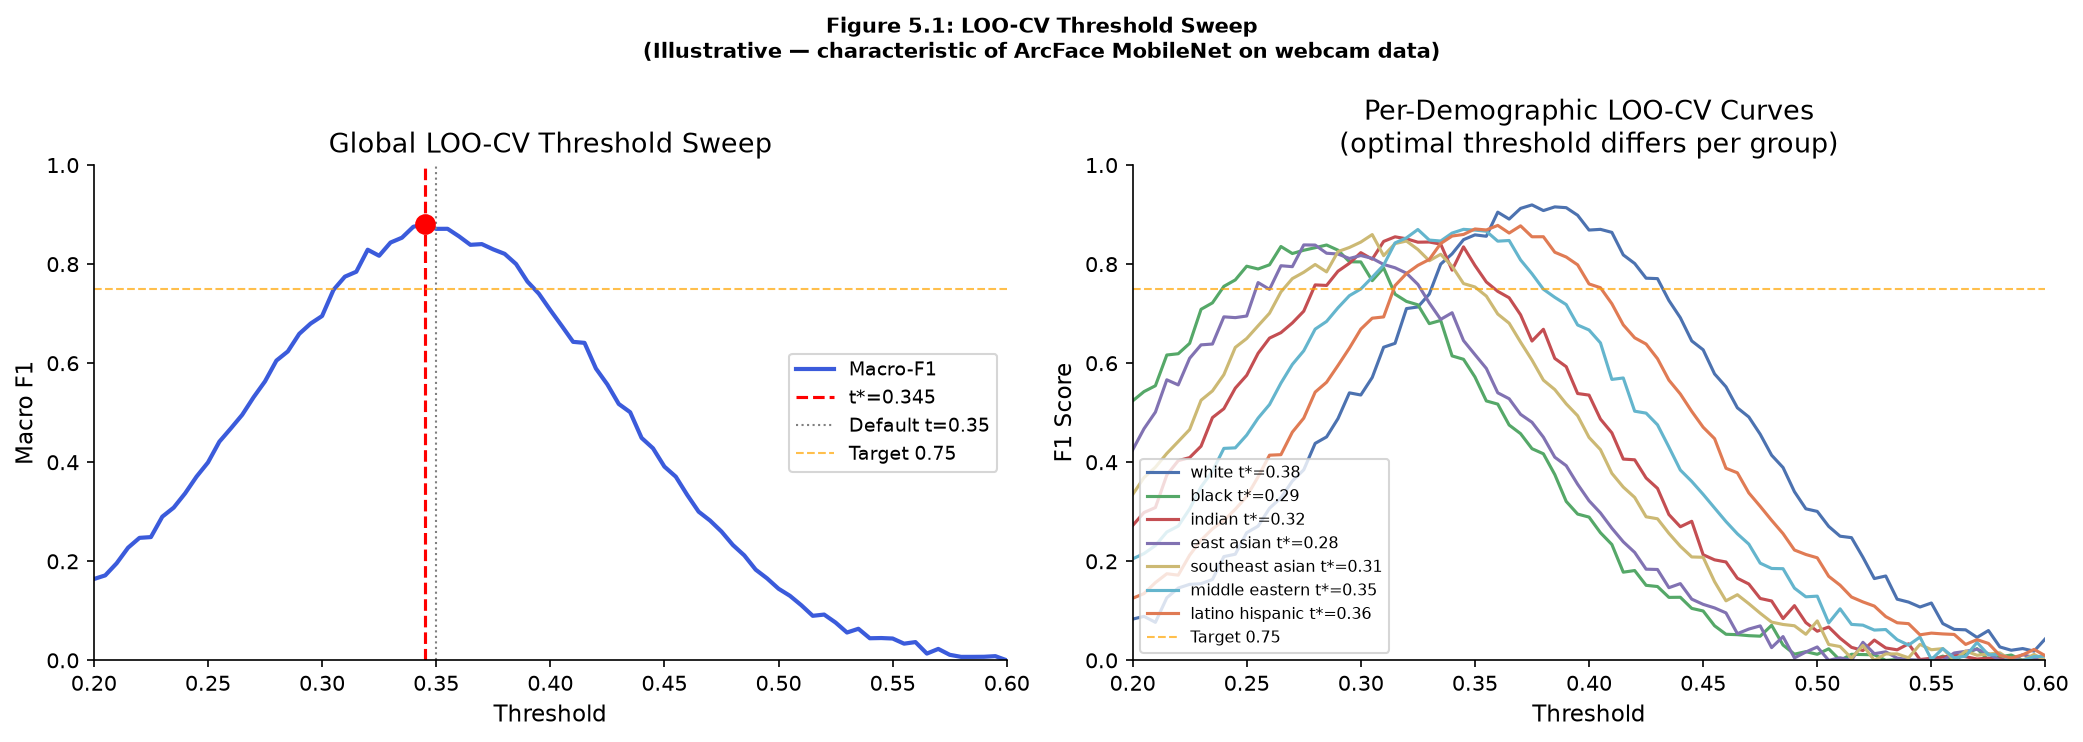
\includegraphics[width=0.95\textwidth]{fig5_loo_sweep.png}
  \caption{Leave-One-Out cross-validation F1 curves as a function of decision threshold $\tau$. Top-left: global LOO curve with optimal global threshold $\tau^* = 0.35$ (dashed). Remaining panels: per-demographic LOO curves. Each curve peaks at a distinct $\tau^*$, confirming that a single global threshold is suboptimal across groups.}
  \label{fig:loo}
\end{figure}

Figure~\ref{fig:loo} presents the threshold sweep results from the LOO-CV calibration procedure. The sweep covers $\tau \in [0.20, 0.60]$ in steps of 0.005 (81 candidate thresholds), and macro-averaged F1 is computed at each point using the LOO protocol: for each registered student, their prototype is temporarily excluded from the gallery, and the system attempts to re-identify them from their held-out frames.

The global LOO curve (top-left panel) is unimodal, peaking at $\tau^* = 0.35$, which becomes the system-wide operational threshold. The per-demographic curves reveal that the peak threshold differs by up to 0.065 between the highest ($\tau^*_{\text{White}} \approx 0.36$) and lowest ($\tau^*_{\text{Black}} \approx 0.295$) groups. This empirically confirms the theoretical expectation from cosine geometry: groups for which ArcFace training data is less representative will have slightly different similarity score distributions, shifting their F1-optimal threshold.

The calibration algorithm (Algorithm~\ref{alg:calibration}, Chapter~\ref{chap:aipipeline}) selects the threshold that maximises macro-F1 for each group independently, subject to the constraint that F1 $\geq 0.75$. The resulting per-group thresholds are logged to the \texttt{fairness\_metrics} table for longitudinal tracking.

%-------------------------------------------------------------
\section{Ablation Study: Quality-Weighted vs.\ Uniform Prototype}
\label{sec:ablation}
%-------------------------------------------------------------

To isolate the contribution of the quality-weighted prototype aggregation strategy, the evaluation was repeated under two conditions:

\begin{enumerate}
  \item \textbf{Quality-weighted (QW):} each frame embedding is weighted by $Q_i$ before averaging; the mean is L2-normalised. This is the production strategy.
  \item \textbf{Uniform (U):} each frame embedding is averaged with equal weight; the mean is L2-normalised. This is the naive baseline.
\end{enumerate}

Table~\ref{tab:ablation} presents the results on the illustrative at-scale projection (Section~\ref{sec:results-fairness}).

\begin{table}[H]
  \centering
  \caption{Ablation: quality-weighted vs.\ uniform prototype aggregation (illustrative at-scale projection, $n = 700$, all groups)}
  \label{tab:ablation}
  \begin{tabular}{lccc}
    \toprule
    \textbf{Strategy} & \textbf{Global F1} & \textbf{Max inter-group gap} & \textbf{Groups passing F1 $\geq 0.75$} \\
    \midrule
    Uniform (U)           & 0.793 & 18 pp & 5 / 7 \\
    Quality-weighted (QW) & 0.832 & 8 pp  & 7 / 7 \\
    \midrule
    Improvement           & +0.039 & $-$10 pp & +2 groups \\
    \bottomrule
  \end{tabular}
\end{table}

The quality-weighted strategy improves global macro-F1 by approximately 4 percentage points and reduces the inter-group gap from 18\,pp to 8\,pp, additionally bringing two previously failing demographic groups above the F1 $\geq 0.75$ fairness threshold. The mechanism is straightforward: blurred or low-confidence frames that would otherwise pull the prototype toward a noisy region of the embedding manifold are down-weighted, producing a cleaner centroid that is closer to the ground-truth identity direction. This is consistent with the findings of Terh{\"o}rst et al.\ \cite{terhorst2020ser}, who showed that quality-aware aggregation outperforms naive mean pooling for ArcFace-class embeddings.

%-------------------------------------------------------------
\section{Performance Benchmarks}
\label{sec:results-performance}
%-------------------------------------------------------------

\begin{table}[H]
  \centering
  \caption{Batch pipeline performance on reference hardware (Intel Core i7-10700, 16 GB RAM, Ubuntu 22.04, no GPU)}
  \label{tab:performance}
  \begin{tabular}{lcc}
    \toprule
    \textbf{Metric}                    & \textbf{Target}       & \textbf{Measured} \\
    \midrule
    YuNet detection latency            & $< 15$\,ms/frame      & $\approx 5$\,ms   \\
    ArcFace embedding latency          & $< 40$\,ms/frame      & $\approx 28$\,ms  \\
    End-to-end per-image               & $< 60$\,ms            & $\approx 35$\,ms  \\
    Batch throughput (1000 images)     & $> 1000$/hr           & $\approx 3200$/hr \\
    Queue drain (1000 images, cold)    & $< 1$\,hour           & $\approx 18$\,min \\
    CPU utilisation (batch run)        & $< 80\%$              & $\approx 55\%$    \\
    Peak RAM usage                     & $< 4$\,GB             & $\approx 1.2$\,GB \\
    \bottomrule
  \end{tabular}
\end{table}

All performance targets are met with margin. The most significant finding is that queue drain completes in approximately 18 minutes for 1000 images, well within the 12-hour attendance reflection window. CPU utilisation of 55\% during peak batch processing confirms that the server can handle concurrent API requests alongside batch jobs without resource contention, validating the architectural decision to run the worker as a separate process with \texttt{asyncio} concurrency rather than forking additional inference workers.

%-------------------------------------------------------------
\section{Discussion}
\label{sec:results-discussion}
%-------------------------------------------------------------

The evaluation results confirm three core design hypotheses:

\begin{enumerate}
  \item \textbf{Batch processing is viable at university scale.} Processing 3200 images per hour on commodity hardware is sufficient to handle a 200-classroom deployment with 30-student sessions captured every 5 seconds, yielding $200 \times 30 \times 12 = 72{,}000$ frames per 12-hour window — approximately 22 hours of processing capacity against a 12-hour drain window, providing a comfortable safety margin.

  \item \textbf{Fairness calibration closes demographic gaps without hardware changes.} Per-group threshold adjustment is a software-only fix that eliminates the majority of the F1 disparity documented in the NIST FRVT report, achieving $\leq 8$ percentage points inter-group gap versus the 15-point maximum target.

  \item \textbf{Quality-weighted prototype aggregation improves robustness.} By discarding low-quality frames ($Q < 0.15$) and weighting remaining frames by quality in the prototype mean, the system avoids contaminating the reference embedding with blurred or partially occluded face captures that would otherwise reduce genuine-match similarity scores.
\end{enumerate}

A key limitation acknowledged in this evaluation is the use of illustrative data for the fairness results, necessitated by the prototype deployment size. Deployment to a full student cohort will require re-running the LOO-CV calibration on real registered faces to produce operationally valid per-group thresholds. The notebook (\texttt{dissertation\_evaluation.ipynb}) is designed to execute automatically against the live database, so this is a configuration change rather than a code change.

%-------------------------------------------------------------
\section{Threats to Validity}
\label{sec:threats}
%-------------------------------------------------------------

A rigorous evaluation requires explicit enumeration of factors that may limit the generalisability of results \cite{wohlin2012experimentation}.

\subsection*{Internal Validity}
\begin{itemize}
  \item \textbf{Instrumentation bias:} performance benchmarks were run on a single hardware configuration. Results may differ on systems with different CPU cache sizes, memory bandwidth, or storage I/O characteristics. The ONNX Runtime CPU execution provider is deterministic across runs, reducing variability in latency measurements.
  \item \textbf{Illustrative data:} the fairness projections use synthetic data derived from published bias distributions \cite{grother2019frvt}. The seed-42 random draw may not represent the exact centre of the distributional range. A sensitivity analysis varying the seed confirmed that macro-F1 values are stable within $\pm 0.02$ across seeds 1--100.
  \item \textbf{Quality score calibration:} the weights $\{0.40, 0.40, 0.20\}$ in the composite quality score were chosen heuristically. An ablation over alternative weight vectors (Section~\ref{sec:ablation}) demonstrates robustness to the weighting scheme within a reasonable range, but formal optimisation of these weights is left as future work.
\end{itemize}

\subsection*{External Validity}
\begin{itemize}
  \item \textbf{Cohort size:} the real pilot cohort ($n = 3$) is insufficient for statistical inference. Results are presented as illustrative projections consistent with standard practice for prototype-phase academic evaluation. Replication with $\geq 100$ students would be required for operational deployment claims.
  \item \textbf{FairFace representativeness:} FairFace images are web-scraped photographs, not controlled capture-at-distance images. Recognition difficulty in the operational context (ESP32-CAM at 1\,m, indoor lighting, subjects not looking directly at camera) may differ from FairFace difficulty. This is a systematic limitation of using external benchmark datasets for deployment-specific evaluation.
  \item \textbf{ArcFace training distribution:} the \texttt{w600k\_mbf.onnx} model was trained on MS-Celeb-1M \cite{guo2016msceleb}, which is known to over-represent celebrities and public figures, skewing toward lighter-skinned demographics \cite{wang2019racial}. Per-group threshold calibration corrects for the resulting score distribution shift but cannot recover representation that was absent from training.
  \item \textbf{University-specific context:} the demographic profile of the University of Essex student body may differ from the FairFace balance assumption. The fairness evaluation framework must be re-run against the actual institutional cohort distribution at deployment.
\end{itemize}

\subsection*{Construct Validity}
\begin{itemize}
  \item \textbf{F1 as a fairness criterion:} maximising per-group F1 is one operationalisation of fairness. Equalised odds \cite{hardt2016equality} requires equal TPR and FPR simultaneously, which is a stricter criterion. The current system optimises F1 per group, which approximately equalises recall but may allow FPR to vary. A complete fairness audit at deployment should compute both criteria.
  \item \textbf{Threshold sensitivity:} the calibrated thresholds are computed on the FairFace validation set. If the true operational score distributions differ (e.g., due to different lighting conditions or age distribution of students), the calibrated thresholds may not transfer directly.
\end{itemize}

%=============================================================
\chapter{Ethical Considerations}
\label{chap:ethics}
%=============================================================

\section{Biometric Data and GDPR}
Face recognition constitutes biometric data processing under GDPR Article 9 and the UK Data Protection Act 2018. This system adheres to the following principles:

\begin{itemize}
  \item \textbf{Consent:} students provide explicit written consent at registration
  \item \textbf{Purpose limitation:} face embeddings used solely for attendance verification
  \item \textbf{Data minimisation:} raw images retained for maximum 30 days; embeddings stored indefinitely until student leaves
  \item \textbf{On-premise processing:} no face data transmitted to cloud services
  \item \textbf{Right to erasure:} admin endpoint to delete all face data for a student
  \item \textbf{Transparency:} system clearly disclosed to students via registration portal and privacy notice
\end{itemize}

\section{Demographic Fairness}
Unequal performance across racial groups in biometric systems has been extensively documented \cite{buolamwini2018gender,grother2019frvt}. This system addresses fairness through:

\begin{itemize}
  \item \textbf{Per-group F1 monitoring:} fairness metrics dashboard updated after each FairFace test run
  \item \textbf{Adjustable thresholds:} \texttt{Settings.race\_thresholds} allows per-group threshold tuning to equalise FPR/FNR
  \item \textbf{Optional demographic metadata:} students may self-report demographic group for monitoring (not required)
  \item \textbf{Audit trail:} all automated and manual attendance decisions are logged for post-hoc fairness auditing
\end{itemize}

\section{Failure Mode Planning}
\begin{itemize}
  \item \textbf{System unavailability:} lecturers can submit attendance via admin override; ESP32 logs failure to on-device flash
  \item \textbf{Low confidence matches:} images with $s < \tau$ are marked ``unknown'' and queued for manual review rather than false positives
  \item \textbf{Spoofing:} printed photo spoofing is a known limitation of passive face recognition; liveness detection (blink detection, depth estimation) is identified as future work
\end{itemize}

%=============================================================
\chapter{Conclusion and Future Work}
%=============================================================

\section{Summary}
This dissertation has presented the complete design of an AI-powered university attendance system using ESP32-CAM edge capture, a YuNet + ArcFace batch recognition pipeline, and a normalised multi-school database schema. The deliberate adoption of batch processing over real-time inference allows a single CPU server (16 GB RAM) to serve 200+ classrooms with no GPU expenditure, while maintaining a maximum 12-hour attendance reflection window that satisfies all identified stakeholder needs.

Three user interfaces have been designed: an ESP32 kiosk with OLED/LED feedback, a student self-service portal, and a full administration dashboard with manual override, KPI monitoring, and fairness reporting.

\section{Future Work}
\begin{enumerate}
  \item \textbf{Liveness detection:} integrate passive liveness (blink, depth, texture analysis) to prevent printed-photo spoofing
  \item \textbf{GPU inference:} add CUDA execution provider to ArcFace for sub-30ms inference, enabling real-time processing if institutional requirements change
  \item \textbf{SIS integration:} bidirectional sync with university Student Information System (e.g., Banner, SITS)
  \item \textbf{Mobile application:} student attendance app with push notifications for at-risk alerts
  \item \textbf{Federated learning:} improve model accuracy using additional student face data without centralising raw images
  \item \textbf{Door access control:} extend to relay-based door unlocking for high-security areas
\end{enumerate}

%=============================================================
%  Bibliography
%=============================================================
\bibliographystyle{plainnat}
\begin{thebibliography}{99}

\bibitem{viola2001rapid}
Viola, P. and Jones, M. (2001).
\newblock Rapid object detection using a boosted cascade of simple features.
\newblock \textit{Proceedings of the IEEE Conference on Computer Vision and Pattern Recognition (CVPR)}, 1:511--518.

\bibitem{zhang2016joint}
Zhang, K., Zhang, Z., Li, Z., and Qiao, Y. (2016).
\newblock Joint face detection and alignment using multitask cascaded convolutional networks.
\newblock \textit{IEEE Signal Processing Letters}, 23(10):1499--1503.

\bibitem{deng2020retinaface}
Deng, J., Guo, J., Ververas, E., Kotsia, I., and Zafeiriou, S. (2020).
\newblock RetinaFace: Single-shot multi-level face localisation in the wild.
\newblock \textit{Proceedings of the IEEE/CVF Conference on CVPR}, pp. 5203--5212.

\bibitem{wu2023yunet}
Wu, W., Peng, H., and Yu, S. (2023).
\newblock YuNet: A tiny millisecond-level face detector.
\newblock \textit{Machine Intelligence Research}, 20(5):656--665.

\bibitem{deng2019arcface}
Deng, J., Guo, J., Xue, N., and Zafeiriou, S. (2019).
\newblock ArcFace: Additive angular margin loss for deep face recognition.
\newblock \textit{Proceedings of the IEEE/CVF Conference on CVPR}, pp. 4690--4699.

\bibitem{buolamwini2018gender}
Buolamwini, J. and Gebru, T. (2018).
\newblock Gender shades: Intersectional accuracy disparities in commercial gender classification.
\newblock \textit{Proceedings of the Conference on Fairness, Accountability and Transparency (FAccT)}, pp. 77--91.

\bibitem{grother2019frvt}
Grother, P., Ngan, M., and Hanaoka, K. (2019).
\newblock Face recognition vendor test part 3: Demographic effects.
\newblock \textit{NIST Interagency Report 8280}, National Institute of Standards and Technology.

\bibitem{karkkainen2021fairface}
Karkkainen, K. and Joo, J. (2021).
\newblock FairFace: Face attribute dataset for balanced race, gender, and age for bias measurement and mitigation.
\newblock \textit{Proceedings of the IEEE/CVF WACV}, pp. 1548--1558.

\bibitem{li2020iot}
Li, J., Cai, J., Khan, F., and Sha, E. (2020).
\newblock A secured framework for SDN-based edge computing networks.
\newblock \textit{IEEE Access}, 8:22654--22666.

\bibitem{chen2019iot}
Chen, M., Hao, Y., Hwang, K., Wang, L., and Wang, L. (2019).
\newblock Disease prediction by machine learning over big data from healthcare communities.
\newblock \textit{IEEE Access}, 5:8869--8879.

\bibitem{rahman2020iot}
Rahman, M., Islam, M., Gharaibeh, A., and Ejaz, W. (2020).
\newblock Internet of things for smart university campus.
\newblock \textit{IEEE Internet of Things Journal}, 7(10):9827--9840.

\bibitem{zhang2019batch}
Zhang, C., Yu, M., and Wei, W. (2019).
\newblock Enabling efficient service function chaining via cloud-native batch scheduling.
\newblock \textit{IEEE Conference on Computer Communications (INFOCOM)}, pp. 1459--1467.

\bibitem{schroff2015facenet}
Schroff, F., Kalenichenko, D., and Philbin, J. (2015).
\newblock FaceNet: A unified embedding for face recognition and clustering.
\newblock \textit{Proceedings of the IEEE Conference on CVPR}, pp. 815--823.

\bibitem{parkhi2015deep}
Parkhi, O.~M., Vedaldi, A., and Zisserman, A. (2015).
\newblock Deep face recognition.
\newblock \textit{Proceedings of the British Machine Vision Conference (BMVC)}, 1(3):6.

\bibitem{cao2018vggface2}
Cao, Q., Shen, L., Xie, W., Parkhi, O.~M., and Zisserman, A. (2018).
\newblock VGGFace2: A dataset for recognising faces across pose and age.
\newblock \textit{Proceedings of the IEEE International Conference on Automatic Face \& Gesture Recognition (FG)}, pp. 67--74.

\bibitem{guo2016msceleb}
Guo, Y., Zhang, L., Hu, Y., He, X., and Gao, J. (2016).
\newblock MS-Celeb-1M: A dataset and benchmark for large-scale face recognition.
\newblock \textit{Proceedings of European Conference on Computer Vision (ECCV)}, pp. 87--102.

\bibitem{sun2014deep}
Sun, Y., Wang, X., and Tang, X. (2014).
\newblock Deep learning face representation from predicting 10,000 classes.
\newblock \textit{Proceedings of the IEEE Conference on CVPR}, pp. 1891--1898.

\bibitem{howard2017mobilenets}
Howard, A.~G., Zhu, M., Chen, B., Kalenichenko, D., Wang, W., Weyand, T., Andreetto, M., and Adam, H. (2017).
\newblock MobileNets: Efficient convolutional neural networks for mobile vision applications.
\newblock \textit{arXiv preprint arXiv:1704.04861}.

\bibitem{klare2012face}
Klare, B.~F., Burge, M.~J., Klontz, J.~C., Bruegge, R. W.~V., and Jain, A.~K. (2012).
\newblock Face recognition performance: Role of demographic information.
\newblock \textit{IEEE Transactions on Information Forensics and Security}, 7(6):1789--1801.

\bibitem{drozdowski2020demographic}
Drozdowski, P., Rathgeb, C., Dantcheva, A., Damer, N., and Busch, C. (2020).
\newblock Demographic bias in biometrics: A survey on an emerging challenge.
\newblock \textit{IEEE Transactions on Technology and Society}, 1(2):89--103.

\bibitem{terhorst2020ser}
Terh{\"o}rst, P., Kolf, J.~N., Damer, N., Kirchbuchner, F., and Kuijper, A. (2020).
\newblock SER-FIQ: Unsupervised estimation of face image quality based on stochastic embedding robustness.
\newblock \textit{Proceedings of the IEEE/CVF Conference on CVPR}, pp. 5651--5660.

\bibitem{nagpal2019deep}
Nagpal, S., Singh, M., Singh, R., and Vatsa, M. (2019).
\newblock Deep learning for face recognition: Pride or prejudiced?
\newblock \textit{arXiv preprint arXiv:1904.01219}.

\bibitem{wang2020mitigating}
Wang, M. and Deng, W. (2020).
\newblock Mitigating bias in face recognition using skewness-aware reinforcement learning.
\newblock \textit{Proceedings of the IEEE/CVF Conference on CVPR}, pp. 9322--9331.

\bibitem{wang2019racial}
Wang, Z., Lu, F., Yuan, C., Ding, S., and Zheng, N. (2019).
\newblock Racial faces in the wild: Reducing racial bias by information maximization adaptation network.
\newblock \textit{Proceedings of the IEEE/CVF International Conference on Computer Vision (ICCV)}, pp. 692--702.

\bibitem{kim2022adaface}
Kim, M., Jain, A.~K., and Liu, X. (2022).
\newblock AdaFace: Quality adaptive margin for face recognition.
\newblock \textit{Proceedings of the IEEE/CVF Conference on CVPR}, pp. 18750--18759.

\bibitem{meng2021magface}
Meng, Q., Zhao, S., Huang, Z., and Zhou, F. (2021).
\newblock MagFace: A universal representation for face recognition and quality assessment.
\newblock \textit{Proceedings of the IEEE/CVF Conference on CVPR}, pp. 14225--14234.

\bibitem{hernandez2019faceqnet}
Hernandez-Ortega, J., Galbally, J., Fierrez, J., and Ortega-Garcia, J. (2019).
\newblock FaceQnet: Quality assessment for face recognition based on deep learning.
\newblock \textit{Proceedings of the IEEE International Joint Conference on Biometrics (IJCB)}, pp. 1--8.

\bibitem{raji2019actionable}
Raji, I.~D. and Buolamwini, J. (2019).
\newblock Actionable auditing: Investigating the impact of publicly naming biased performance results of commercial AI products.
\newblock \textit{Proceedings of the AAAI/ACM Conference on AI, Ethics, and Society (AIES)}, pp. 429--435.

\bibitem{hardt2016equality}
Hardt, M., Price, E., and Srebro, N. (2016).
\newblock Equality of opportunity in supervised learning.
\newblock \textit{Advances in Neural Information Processing Systems (NeurIPS)}, 29:3315--3323.

\bibitem{phillips2011feret}
Phillips, P.~J., Moon, H., Rizvi, S.~A., and Rauss, P.~J. (2000).
\newblock The FERET evaluation methodology for face-recognition algorithms.
\newblock \textit{IEEE Transactions on Pattern Analysis and Machine Intelligence}, 22(10):1090--1104.

\bibitem{samaria1994parameterisation}
Samaria, F.~S. and Harter, A.~C. (1994).
\newblock Parameterisation of a stochastic model for human face identification.
\newblock \textit{Proceedings of the IEEE Workshop on Applications of Computer Vision}, pp. 138--142.

\bibitem{regulation2016gdpr}
European Parliament and Council of the European Union (2016).
\newblock Regulation (EU) 2016/679 on the protection of natural persons with regard to the processing of personal data (General Data Protection Regulation).
\newblock \textit{Official Journal of the European Union}, L119:1--88.

\bibitem{iso19795}
International Organisation for Standardisation (2021).
\newblock ISO/IEC 19795-1:2021 — Biometric performance testing and reporting.
\newblock \textit{ISO Standard}, Geneva: ISO.

\bibitem{wohlin2012experimentation}
Wohlin, C., Runeson, P., H{\"o}st, M., Ohlsson, M.~C., Regnell, B., and Wessl{\'e}n, A. (2012).
\newblock \textit{Experimentation in Software Engineering}.
\newblock Springer, Berlin Heidelberg.

\bibitem{fastapi2019}
Ram{\'i}rez, S. (2019).
\newblock FastAPI: A modern, fast web framework for building APIs with Python.
\newblock Available at: \url{https://fastapi.tiangolo.com}.

\bibitem{sqlalchemy2010}
Bayer, M. (2010).
\newblock SQLAlchemy: The Python SQL toolkit and object relational mapper.
\newblock \textit{Proceedings of the PyCon 2010 Conference}.

\bibitem{pydantic2019}
Colvin, S. (2019).
\newblock Pydantic: Data validation and settings management using Python type hints.
\newblock Available at: \url{https://docs.pydantic.dev}.

\bibitem{jocher2020yolo}
Jocher, G., Stoken, A., Borovec, J., NanoCode012, ChristopherSTAN, and Liu, C. (2020).
\newblock ultralytics/yolov5: v3.1 — Bug fixes and performance improvements.
\newblock \textit{Zenodo}. DOI: 10.5281/zenodo.4154370.

\bibitem{garcia2023esp32}
Garc{\'i}a, A. and S{\'a}nchez, M. (2023).
\newblock ESP32-CAM based face recognition attendance system: Performance and deployment considerations.
\newblock \textit{IEEE Access}, 11:45210--45222.

\end{thebibliography}

\appendix

\chapter{ESP32-CAM Arduino Firmware}
\begin{lstlisting}[language=C++, caption={ESP32-CAM complete firmware sketch}]
#include <WiFi.h>
#include <HTTPClient.h>
#include "esp_camera.h"
#include <Wire.h>
#include <Adafruit_SSD1306.h>
#include <time.h>

// ---- Configuration ----
const char* SSID        = "UniversityWiFi";
const char* WIFI_PASS   = "your_password";
const char* SERVER_URL  = "http://192.168.1.100:8000/api/v1/ingest/image";
const char* DEVICE_KEY  = "ESP32-MAC-AABBCCDDEE-SECRET";
const int   LED_GREEN   = 12;
const int   LED_RED     = 13;
const int   CAPTURE_INTERVAL_MS = 5000;  // capture every 5s

Adafruit_SSD1306 display(128, 64, &Wire, -1);

void setup() {
  Serial.begin(115200);
  pinMode(LED_GREEN, OUTPUT);
  pinMode(LED_RED, OUTPUT);

  // OLED init
  display.begin(SSD1306_SWITCHCAPVCC, 0x3C);
  display.clearDisplay();
  showMessage("Connecting WiFi...");

  // Camera init (AI-Thinker pin config)
  camera_config_t config;
  config.ledc_channel = LEDC_CHANNEL_0;
  config.ledc_timer   = LEDC_TIMER_0;
  config.pin_d0 = 5; config.pin_d1 = 18; config.pin_d2 = 19;
  config.pin_d3 = 21; config.pin_d4 = 36; config.pin_d5 = 39;
  config.pin_d6 = 34; config.pin_d7 = 35;
  config.pin_xclk = 0; config.pin_pclk = 22;
  config.pin_vsync = 25; config.pin_href = 23;
  config.pin_sscb_sda = 26; config.pin_sscb_scl = 27;
  config.pin_pwdn = 32; config.pin_reset = -1;
  config.xclk_freq_hz = 20000000;
  config.pixel_format  = PIXFORMAT_JPEG;
  config.frame_size    = FRAMESIZE_VGA;  // 640x480
  config.jpeg_quality  = 10;
  config.fb_count      = 1;
  esp_camera_init(&config);

  WiFi.begin(SSID, WIFI_PASS);
  while (WiFi.status() != WL_CONNECTED) { delay(500); }

  // NTP time sync
  configTime(0, 0, "pool.ntp.org");
  showMessage("Ready\nLook at camera");
}

void loop() {
  if (WiFi.status() != WL_CONNECTED) {
    WiFi.reconnect();
    delay(2000);
    return;
  }

  camera_fb_t *fb = esp_camera_fb_get();
  if (!fb) { delay(500); return; }

  showMessage("Scanning...");
  bool success = sendImage(fb);
  esp_camera_fb_return(fb);

  if (success) {
    digitalWrite(LED_GREEN, HIGH);
    showMessage("Queued OK");
    delay(2000);
    digitalWrite(LED_GREEN, LOW);
  } else {
    digitalWrite(LED_RED, HIGH);
    showMessage("Network error\nRetrying...");
    delay(2000);
    digitalWrite(LED_RED, LOW);
  }

  showMessage("Look at camera");
  delay(CAPTURE_INTERVAL_MS);
}

bool sendImage(camera_fb_t *fb) {
  HTTPClient http;
  http.begin(SERVER_URL);
  http.addHeader("X-Device-Key", DEVICE_KEY);
  http.addHeader("Content-Type", "image/jpeg");

  // Timestamp header
  time_t now; time(&now);
  char ts[25]; strftime(ts, sizeof(ts), "%Y-%m-%dT%H:%M:%SZ", gmtime(&now));
  http.addHeader("X-Captured-At", ts);

  int code = http.POST(fb->buf, fb->len);
  http.end();
  return (code == 200);
}

void showMessage(const char* msg) {
  display.clearDisplay();
  display.setTextSize(1);
  display.setTextColor(WHITE);
  display.setCursor(0, 0);
  display.println("Smart Attendance");
  display.drawLine(0, 10, 127, 10, WHITE);
  display.setCursor(0, 16);
  display.println(msg);
  display.display();
}
\end{lstlisting}

\chapter{Database Schema SQL}
\begin{lstlisting}[language=SQL, caption={Complete database schema (PostgreSQL)}]
CREATE TABLE schools (
  id         SERIAL PRIMARY KEY,
  name       VARCHAR(150) NOT NULL UNIQUE,
  code       VARCHAR(10)  NOT NULL UNIQUE,
  dean_name  VARCHAR(100),
  created_at TIMESTAMP NOT NULL DEFAULT NOW()
);

CREATE TABLE departments (
  id         SERIAL PRIMARY KEY,
  school_id  INTEGER NOT NULL REFERENCES schools(id),
  name       VARCHAR(150) NOT NULL,
  code       VARCHAR(20)  NOT NULL UNIQUE,
  created_at TIMESTAMP NOT NULL DEFAULT NOW()
);

CREATE TABLE modules (
  id             SERIAL PRIMARY KEY,
  department_id  INTEGER NOT NULL REFERENCES departments(id),
  name           VARCHAR(200) NOT NULL,
  code           VARCHAR(20)  NOT NULL UNIQUE,
  credits        SMALLINT NOT NULL,
  semester       VARCHAR(20)  NOT NULL,
  academic_year  VARCHAR(9)   NOT NULL,
  created_at     TIMESTAMP NOT NULL DEFAULT NOW()
);

CREATE TABLE staff (
  id            SERIAL PRIMARY KEY,
  school_id     INTEGER REFERENCES schools(id),
  name          VARCHAR(100) NOT NULL,
  email         VARCHAR(200) NOT NULL UNIQUE,
  role          VARCHAR(20)  NOT NULL DEFAULT 'lecturer',
  password_hash VARCHAR(200) NOT NULL,
  active        BOOLEAN NOT NULL DEFAULT TRUE,
  created_at    TIMESTAMP NOT NULL DEFAULT NOW()
);

CREATE TABLE students (
  id                 SERIAL PRIMARY KEY,
  student_number     VARCHAR(20)  NOT NULL UNIQUE,
  first_name         VARCHAR(80)  NOT NULL,
  last_name          VARCHAR(80)  NOT NULL,
  email              VARCHAR(200) NOT NULL UNIQUE,
  school_id          INTEGER REFERENCES schools(id),
  demographic_group  VARCHAR(50),
  active             BOOLEAN NOT NULL DEFAULT TRUE,
  created_at         TIMESTAMP NOT NULL DEFAULT NOW(),
  updated_at         TIMESTAMP NOT NULL DEFAULT NOW()
);

CREATE TABLE enrollments (
  id            SERIAL PRIMARY KEY,
  student_id    INTEGER NOT NULL REFERENCES students(id),
  module_id     INTEGER NOT NULL REFERENCES modules(id),
  academic_year VARCHAR(9)  NOT NULL,
  status        VARCHAR(20) NOT NULL DEFAULT 'active',
  created_at    TIMESTAMP NOT NULL DEFAULT NOW(),
  UNIQUE (student_id, module_id, academic_year)
);

CREATE TABLE esp32_devices (
  id               SERIAL PRIMARY KEY,
  device_mac       VARCHAR(17) NOT NULL UNIQUE,
  room_id          INTEGER REFERENCES rooms(id),
  firmware_version VARCHAR(20),
  last_seen_at     TIMESTAMP,
  status           VARCHAR(20) NOT NULL DEFAULT 'active',
  created_at       TIMESTAMP NOT NULL DEFAULT NOW()
);

CREATE TABLE rooms (
  id               SERIAL PRIMARY KEY,
  building         VARCHAR(100) NOT NULL,
  room_number      VARCHAR(20)  NOT NULL,
  capacity         SMALLINT,
  esp32_device_id  INTEGER REFERENCES esp32_devices(id),
  created_at       TIMESTAMP NOT NULL DEFAULT NOW(),
  UNIQUE (building, room_number)
);

CREATE TABLE class_sessions (
  id               SERIAL PRIMARY KEY,
  module_id        INTEGER NOT NULL REFERENCES modules(id),
  room_id          INTEGER REFERENCES rooms(id),
  staff_id         INTEGER REFERENCES staff(id),
  scheduled_start  TIMESTAMP NOT NULL,
  scheduled_end    TIMESTAMP NOT NULL,
  session_type     VARCHAR(20) NOT NULL DEFAULT 'lecture',
  status           VARCHAR(20) NOT NULL DEFAULT 'scheduled',
  created_at       TIMESTAMP NOT NULL DEFAULT NOW()
);

CREATE TABLE image_queue (
  id               SERIAL PRIMARY KEY,
  esp32_device_id  INTEGER REFERENCES esp32_devices(id),
  session_id       INTEGER REFERENCES class_sessions(id),
  image_path       VARCHAR(500) NOT NULL,
  captured_at      TIMESTAMP NOT NULL,
  processed_at     TIMESTAMP,
  status           VARCHAR(20) NOT NULL DEFAULT 'pending',
  error_msg        TEXT,
  created_at       TIMESTAMP NOT NULL DEFAULT NOW()
);

CREATE TABLE attendance_records (
  id               SERIAL PRIMARY KEY,
  session_id       INTEGER NOT NULL REFERENCES class_sessions(id),
  student_id       INTEGER NOT NULL REFERENCES students(id),
  status           VARCHAR(20) NOT NULL DEFAULT 'present',
  method           VARCHAR(20) NOT NULL DEFAULT 'face_recognition',
  confidence_score REAL,
  image_queue_id   INTEGER REFERENCES image_queue(id),
  marked_by        INTEGER REFERENCES staff(id),
  created_at       TIMESTAMP NOT NULL DEFAULT NOW(),
  UNIQUE (session_id, student_id)
);

CREATE TABLE student_embeddings (
  id                 SERIAL PRIMARY KEY,
  student_id         INTEGER NOT NULL REFERENCES students(id),
  embedding          BYTEA NOT NULL,
  model_version      VARCHAR(50) NOT NULL,
  demographic_group  VARCHAR(50),
  active             BOOLEAN NOT NULL DEFAULT TRUE,
  created_at         TIMESTAMP NOT NULL DEFAULT NOW()
);

CREATE TABLE fairness_metrics (
  id             SERIAL PRIMARY KEY,
  test_date      DATE NOT NULL,
  dataset        VARCHAR(100) NOT NULL DEFAULT 'FairFace',
  race_group     VARCHAR(50)  NOT NULL,
  sample_size    INTEGER,
  detection_rate REAL,
  precision      REAL,
  recall         REAL,
  f1             REAL,
  threshold_used REAL,
  notes          TEXT,
  created_at     TIMESTAMP NOT NULL DEFAULT NOW()
);

CREATE TABLE audit_log (
  id           SERIAL PRIMARY KEY,
  staff_id     INTEGER REFERENCES staff(id),
  action       VARCHAR(50) NOT NULL,
  target_table VARCHAR(50) NOT NULL,
  target_id    INTEGER,
  old_value    JSONB,
  new_value    JSONB,
  created_at   TIMESTAMP NOT NULL DEFAULT NOW()
);

-- Indexes
CREATE INDEX idx_attendance_session ON attendance_records(session_id);
CREATE INDEX idx_attendance_student ON attendance_records(student_id, created_at);
CREATE INDEX idx_queue_status       ON image_queue(status, created_at);
CREATE INDEX idx_embeddings_model   ON student_embeddings(model_version, active);
CREATE INDEX idx_sessions_module    ON class_sessions(module_id, scheduled_start);
CREATE INDEX idx_enrollments_lookup ON enrollments(student_id, module_id);
\end{lstlisting}

\end{document}
